% Options for packages loaded elsewhere
\PassOptionsToPackage{unicode}{hyperref}
\PassOptionsToPackage{hyphens}{url}
\documentclass[
  11pt,
]{article}
\usepackage{xcolor}
\usepackage[left=3cm,right=3cm,top=2.5cm,bottom=2.5cm]{geometry}
\usepackage{amsmath,amssymb}
\setcounter{secnumdepth}{5}
\usepackage{iftex}
\ifPDFTeX
  \usepackage[T1]{fontenc}
  \usepackage[utf8]{inputenc}
  \usepackage{textcomp} % provide euro and other symbols
\else % if luatex or xetex
  \usepackage{unicode-math} % this also loads fontspec
  \defaultfontfeatures{Scale=MatchLowercase}
  \defaultfontfeatures[\rmfamily]{Ligatures=TeX,Scale=1}
\fi
\usepackage{lmodern}
\ifPDFTeX\else
  % xetex/luatex font selection
\fi
% Use upquote if available, for straight quotes in verbatim environments
\IfFileExists{upquote.sty}{\usepackage{upquote}}{}
\IfFileExists{microtype.sty}{% use microtype if available
  \usepackage[]{microtype}
  \UseMicrotypeSet[protrusion]{basicmath} % disable protrusion for tt fonts
}{}
\usepackage{setspace}
\makeatletter
\@ifundefined{KOMAClassName}{% if non-KOMA class
  \IfFileExists{parskip.sty}{%
    \usepackage{parskip}
  }{% else
    \setlength{\parindent}{0pt}
    \setlength{\parskip}{6pt plus 2pt minus 1pt}}
}{% if KOMA class
  \KOMAoptions{parskip=half}}
\makeatother
\usepackage{longtable,booktabs,array}
\usepackage{caption}
\captionsetup[table]{skip=6pt}
\newcounter{none} % for unnumbered tables
\usepackage{calc} % for calculating minipage widths
% Correct order of tables after \paragraph or \subparagraph
\usepackage{etoolbox}
\makeatletter
\patchcmd\longtable{\par}{\if@noskipsec\mbox{}\fi\par}{}{}
\makeatother
% Allow footnotes in longtable head/foot
\IfFileExists{footnotehyper.sty}{\usepackage{footnotehyper}}{\usepackage{footnote}}
\makesavenoteenv{longtable}
\usepackage{graphicx}
\makeatletter
\newsavebox\pandoc@box
\newcommand*\pandocbounded[1]{% scales image to fit in text height/width
  \sbox\pandoc@box{#1}%
  \Gscale@div\@tempa{\textheight}{\dimexpr\ht\pandoc@box+\dp\pandoc@box\relax}%
  \Gscale@div\@tempb{\linewidth}{\wd\pandoc@box}%
  \ifdim\@tempb\p@<\@tempa\p@\let\@tempa\@tempb\fi% select the smaller of both
  \ifdim\@tempa\p@<\p@\scalebox{\@tempa}{\usebox\pandoc@box}%
  \else\usebox{\pandoc@box}%
  \fi%
}
% Set default figure placement to htbp
\def\fps@figure{htbp}
\makeatother
% definitions for citeproc citations
\NewDocumentCommand\citeproctext{}{}
\NewDocumentCommand\citeproc{mm}{%
  \begingroup\def\citeproctext{#2}\cite{#1}\endgroup}
\makeatletter
 % allow citations to break across lines
 \let\@cite@ofmt\@firstofone
 % avoid brackets around text for \cite:
 \def\@biblabel#1{}
 \def\@cite#1#2{{#1\if@tempswa , #2\fi}}
\makeatother
\newlength{\cslhangindent}
\setlength{\cslhangindent}{1.5em}
\newlength{\csllabelwidth}
\setlength{\csllabelwidth}{3em}
\newenvironment{CSLReferences}[2] % #1 hanging-indent, #2 entry-spacing
 {\begin{list}{}{%
  \setlength{\itemindent}{0pt}
  \setlength{\leftmargin}{0pt}
  \setlength{\parsep}{0pt}
  % turn on hanging indent if param 1 is 1
  \ifodd #1
   \setlength{\leftmargin}{\cslhangindent}
   \setlength{\itemindent}{-1\cslhangindent}
  \fi
  % set entry spacing
  \setlength{\itemsep}{#2\baselineskip}}}
 {\end{list}}
\usepackage{calc}
\newcommand{\CSLBlock}[1]{\hfill\break\parbox[t]{\linewidth}{\strut\ignorespaces#1\strut}}
\newcommand{\CSLLeftMargin}[1]{\parbox[t]{\csllabelwidth}{\strut#1\strut}}
\newcommand{\CSLRightInline}[1]{\parbox[t]{\linewidth - \csllabelwidth}{\strut#1\strut}}
\newcommand{\CSLIndent}[1]{\hspace{\cslhangindent}#1}
\setlength{\emergencystretch}{3em} % prevent overfull lines
\providecommand{\tightlist}{%
  \setlength{\itemsep}{0pt}\setlength{\parskip}{0pt}}
% Statistics in Medicine submission preamble.
% Shared across analysis/report/<paper>/report.Rmd files via
%   includes:
%     in_header: ../sim-preamble.tex
% in the YAML output block.
%
% The page footer (source path, render time, version) is no
% longer set here. It is supplied at render time by the vendored
% tools/stamp-render.R, which injects tools/stamp.tex.

% Continuous line numbering for editorial review. The 'mathlines'
% option extends numbering through display-math environments
% (equation, align, ...), which SIM editorial workflows expect.
\usepackage[mathlines]{lineno}
\linenumbers
\usepackage{amsmath}

% Spacing: linestretch is set in YAML (1.5 line spacing).
\usepackage{setspace}
%% tools/stamp.tex
%% Provenance footer for PDFs rendered from this project.
%% Vendored by zzcollab; this file is not project-specific. The
%% footer prints the source document and the time of rendering.
%% The git version is defined here too, and so is available to a
%% project that wants it on the page, but it is left off the
%% default footer: it already names the staged copy in share/ and
%% appears in its manifest row. All values are supplied at render
%% time by tools/stamp-render.R, which writes a small generated
%% file that redefines the macros below. The \providecommand
%% defaults keep a bare LaTeX compile working when the document is
%% built without the wrapper.
\usepackage{fancyhdr}
\usepackage{xcolor}
\providecommand{\stampsource}{\detokenize{(source not recorded)}}
\providecommand{\stamptime}{(time not recorded)}
\providecommand{\stampversion}{\detokenize{(version not recorded)}}
\setlength{\footskip}{40pt}
\newcommand{\stampfootcontent}{%
  \footnotesize\color{gray}%
  \parbox[b]{\textwidth}{%
    \stamptime\hfill\thepage\\[2pt]%
    \ttfamily\raggedright\stampsource}}
\pagestyle{fancy}
\fancyhf{}
\fancyfoot[C]{\stampfootcontent}
\renewcommand{\headrulewidth}{0pt}
\renewcommand{\footrulewidth}{0.4pt}
%% The title page uses the `plain` page style; redefine it so the
%% stamp appears there too.
\fancypagestyle{plain}{%
  \fancyhf{}%
  \fancyfoot[C]{\stampfootcontent}%
  \renewcommand{\headrulewidth}{0pt}%
  \renewcommand{\footrulewidth}{0.4pt}}
\renewcommand{\stampsource}{\textasciitilde{}/\allowbreak{}prj/\allowbreak{}res/\allowbreak{}36-pmsimstats-ng/\allowbreak{}pmsimstats-ng/\allowbreak{}analysis/\allowbreak{}report/\allowbreak{}02-carryover-sensitivity/\allowbreak{}report.Rmd}
\renewcommand{\stamptime}{2026-08-18 17:24 PDT}
\renewcommand{\stampversion}{\detokenize{8817308-wip}}
\usepackage{amsmath}
\usepackage{amssymb}
\usepackage{booktabs}
\usepackage{longtable}
\usepackage{float}
\usepackage[mathlines]{lineno}
\linenumbers
\usepackage{booktabs}
\usepackage{longtable}
\usepackage{array}
\usepackage{multirow}
\usepackage{wrapfig}
\usepackage{float}
\usepackage{colortbl}
\usepackage{pdflscape}
\usepackage{tabu}
\usepackage{threeparttable}
\usepackage{threeparttablex}
\usepackage[normalem]{ulem}
\usepackage{makecell}
\usepackage{xcolor}
\usepackage{bookmark}
\IfFileExists{xurl.sty}{\usepackage{xurl}}{} % add URL line breaks if available
\urlstyle{same}
% fallback for those not using the hyperref driver hyperxmp:
\makeatletter
\@ifundefined{xmpquote}{\newcommand{\xmpquote}[1]{#1}}{}
\makeatother
\hypersetup{
  pdftitle={Unadjusted{,} lag-adjusted{,} and exposure-weighted carryover specifications under differential-correlation biomarker interactions: a factorial simulation study},
  pdfauthor={pmsimstats team},
  hidelinks,
  pdfcreator={LaTeX via pandoc}}

\title{Unadjusted, lag-adjusted, and exposure-weighted carryover specifications under differential-correlation biomarker interactions: a factorial simulation study}
\author{pmsimstats team}
\date{August 18, 2026}

\begin{document}
\maketitle

{
\setcounter{tocdepth}{2}
\tableofcontents
}
\setstretch{1.1}
\section*{Abstract}\label{abstract}
\addcontentsline{toc}{section}{Abstract}

\textbf{Background.} Aggregated N-of-1 trials pool repeated within-patient
on/off contrasts to validate predictive biomarkers. Under covariance
moderation, a multivariate-normal differential-correlation
architecture in which the biomarker-treatment interaction lives in a
treatment-state-dependent correlation, a companion study found that
carryover costs up to roughly 31\% of power in relative terms. The
analyst must still decide how to represent residual exposure in the
linear predictor, and it is not established which representation is
most robust to the ordinarily unknown pharmacokinetic decay shape.

\textbf{Methods.} We compare three analysis-model specifications for the
drug-exposure regressor. Unadjusted is the binary on-drug indicator,
ignoring carryover altogether. Lag-adjusted augments that indicator
with a lagged just-off-drug term estimating carryover
non-parametrically, the classical crossover device. Exposure-weighted
is a continuous indicator committing to a parametric decay and
half-life, the current default. We
embed them in an ADEMP-structured factorial simulation\textsuperscript{\citeproc{ref-morris2019simulation}{1}} crossing two DGP decay forms (exponential,
Weibull) with the three specifications, three trial designs, two
sample sizes, and three interaction strengths (216 cells, 500
replicates each), plus four sensitivity blocks and a cluster-robust
recalibration. All three specifications are fitted to the same
simulated datasets, so every contrast is paired, and each
performance measure is reported with its Monte Carlo standard error
(MCSE).

\textbf{Results.} Two findings stand out. First, the lagged-treatment term
buys nothing. Lag-adjusted and Unadjusted are statistically
indistinguishable across all 216 cells, differing by a mean of 0.003
in power against an MCSE of 0.018, and agreeing to three decimal
places on bias, mean squared error, and coverage. Because the two
share an estimand and differ by exactly one nuisance term, this is a
clean null. Second, Exposure-weighted attains the highest power only
in the two designs with a blinded-discontinuation phase (Hybrid and
OL+BDC), where its advantage is about 10 percentage points (0.860 vs
0.766 for Unadjusted at the reference cell). Under the classical
crossover (CO) design it is markedly inferior (0.488 vs 0.830).
Where it leads, the lead is robust to decay-shape and half-life
mis-specification and to autocorrelation strength. The model-based
interaction test is mildly conservative for all three (mean null
rejection 0.036 to 0.039), an artifact of the working covariance that
a CR2 cluster-robust standard error removes without disturbing the
ranking.

\textbf{Conclusions.} Three points warrant emphasis. First, under the
covariance-moderation architecture we recommend the exposure-weighted
predictor, reported with a cluster-robust standard error, for the
Hybrid and OL+BDC designs. Under a crossover design it should not be
used, and the unadjusted binary indicator is materially better.
Second, the classical lagged-treatment remedy cannot be recommended
in any design examined here, since it never improved on ignoring
carryover altogether. We trace this to its entering the model as a
nuisance main effect, which leaves the attenuation of the interaction
untouched. Third, across all conditions anticipated dropout governs
power far more than the choice among specifications, and should
dominate design effort accordingly. This manuscript restricts the
grid to the covariance-moderation architecture and to the exponential
and Weibull decay forms. The mean-moderation architecture and linear
decay are evaluated in the archived companion drafts
\texttt{archive/report.Rmd} and \texttt{archive/report-slim.Rmd}.

\section{Introduction}\label{introduction}

In a single N-of-1 trial, one patient is crossed repeatedly between
active treatment and a comparator, and the within-patient contrast
between on-drug and off-drug periods estimates that patient's
individual treatment effect. An aggregated N-of-1 trial pools many
such series into a mixed model, trading some within-patient
resolution for population-level inference at sample sizes
considerably smaller than a parallel-group trial would require\textsuperscript{\citeproc{ref-hendrickson2020}{2}}. The estimand is the biomarker-treatment
interaction, whether a baseline covariate \(B_i\) modifies the
treatment effect. We examine three trial designs that differ in how
on-drug and off-drug occasions are arranged, a classical crossover
(CO), an open-label design followed by blinded discontinuation
(OL+BDC), and a Hybrid N-of-1 design, each defined in Section 2.2.

The inferential complication specific to this setting is carryover.
A drug's pharmacological effect does not switch off abruptly at
discontinuation but decays over days or weeks, so nominally off-drug
observations still carry residual exposure. An exposure regressor
that ignores this is a mis-measured version of what the patient
actually received, and the damage is twofold. The interaction
contrast is diluted, because occasions still carrying a substantial
fraction of the drug effect are coded identically to occasions
carrying none, biasing the biomarker-by-exposure coefficient toward
zero as any covariate measured with error would. And those same
occasions are heterogeneous in a way the model does not represent,
so the unexplained variation inflates the standard error of the
coefficient that has just been attenuated. The test loses on both
counts, and power falls accordingly.

This is a loss of power, not of validity. Under the null, \(c_{bm} =
0\), no biomarker-response association exists at any level of
residual exposure, so a mis-coded regressor has no interaction to
distort and test size is unaffected by exposure coding. The mild
conservatism observed in Section 3.5 has a separate origin in the
working covariance and applies equally across specifications.
Carryover mis-specification is therefore a question of efficiency,
and we frame the study in terms of recovered power.

Three answers are available for how to represent residual exposure
in the linear predictor, corresponding to three positions an analyst
can take toward the unknown decay. The analyst may deny it, coding
exposure strictly on or off, may estimate it, adding a nuisance term
whose magnitude the data determine, or may assume it, committing to a
decay curve and a half-life. A companion study\textsuperscript{\citeproc{ref-pmsimstats_dgp_architectures2026}{3}},
building on Hendrickson\textsuperscript{\citeproc{ref-hendrickson2020}{2}}, shows that under the
covariance-moderation architecture, in which the interaction lives
in the treatment-state-dependent covariance \(\text{Cor}(B_i,
BR_{it}) = c_{bm} \cdot \phi(t_{sd})\), carryover erodes power
directly and design-dependently. At a half-life of one week, the
relative loss is roughly 31\% under OL+BDC but only 3 to 5\% under
crossover and Hybrid, against 1 to 3\% under an alternative
architecture where the biomarker moderates the mean response
directly. We restrict attention here to covariance moderation, where
the carryover problem is largest and Hendrickson's original results
were obtained. That earlier work fixed the decay shape at
exponential and evaluated only one analysis specification, leaving
open which representation of residual exposure performs best when
the true decay shape is not known precisely, as is ordinarily the
case.

We compare three specifications. Unadjusted is the binary on-drug
indicator, ignoring carryover entirely and serving as the benchmark
any remedy must beat. Lag-adjusted augments it with a lagged
just-off-drug term that estimates carryover magnitude without
assuming a functional form, following the classical crossover-trial
device of Jones and Kenward\textsuperscript{\citeproc{ref-jones2014crossover}{4}}. Exposure-weighted
is a continuous indicator committing to a parametric decay form and
half-life, the current pmsimstats-ng default. Unadjusted and
Lag-adjusted estimate the same coefficient and are fitted to the
same simulated datasets, differing by exactly one nuisance term, so
their contrast isolates that term's contribution alone.
Exposure-weighted differs on a second axis as well, since it changes
the regressor carrying the interaction. We cross all three against
exponential and Weibull data-generating decay forms and ask whether
one can be recommended outright, or whether the choice depends on
trial design, following the ADEMP reporting framework of Morris,
White, and Crowther\textsuperscript{\citeproc{ref-morris2019simulation}{1}} throughout. Section 2
describes the simulation design in ADEMP order, Section 3 gives the
results, and Section 4 takes up the practical implications.

\section{Simulation design}\label{simulation-design}

The study simulates complete aggregated N-of-1 trials and analyzes
each one under every specification. A single replicate proceeds as
follows. Patients are allocated across the randomization paths of the
chosen trial design (Section 2.2). For each patient we draw a
pre-treatment biomarker together with the three latent response
components, namely the pharmacological response, the natural-history
trend and the placebo-belief component, jointly across all eight
measurement occasions from a multivariate normal distribution whose
means follow modified Gompertz trajectories and whose covariance
carries within-component AR(1) autocorrelation, cross-component
correlations, and the treatment-state-dependent biomarker-response
correlation that encodes the interaction (Section 2.3). The observed
symptom score at each occasion is the patient's baseline severity
less the sum of the three components, so that a beneficial effect
lowers the score. Carryover enters through a decay function of time
since discontinuation, which keeps part of the pharmacological effect
present at nominally off-drug occasions. All three analysis
specifications (Section 2.4) are then fitted to that same simulated
dataset, and we record the interaction coefficient, its standard
error and its \(p\)-value from each. This is repeated 500 times for
every parameter combination in the grid of Section 2.5.

Fitting all specifications to a common dataset is deliberate. It
makes every contrast among them paired, so that differences are
estimated with substantially less Monte Carlo variance than
independent draws would give. Throughout, \(N\) denotes the \textbf{total}
number of patients in a trial, allocated as evenly as possible across
the design's randomization paths, so a design with \(P\) paths assigns
about \(N/P\) patients to each. At \(N = 70\) this is 35 per path under
the two-path designs and 17 or 18 per path under the four-path Hybrid
design.

\subsection{Aims}\label{aims}

The aim is to quantify, under covariance moderation, the cost of
mis-specifying the carryover representation in the analysis model,
and to determine which of the three candidate strategies performs
better across the grid of data-generating decay forms and trial
designs. A second aim, addressed in the Tier 2 sensitivity blocks of
Section 3.6, is to check whether the resulting ranking survives
perturbation of within-subject autocorrelation, dropout rate,
half-life accuracy, and interaction size.

\subsection{Trial designs}\label{trial-designs}

The three designs differ in how on-drug and off-drug occasions are
arranged, and so in how much post-discontinuation information each
generates. All three schedule eight measurement occasions per
patient across randomization paths, each a fixed on-drug/off-drug
schedule, and each design carries an expectancy weight (one during
open-label periods, one half during blinded periods) scaling the
placebo-belief component.

\textbf{Crossover (CO).} A traditional two-period within-patient
crossover, blinded throughout, occasions spaced 2.5 weeks apart from
2.5 to 20 weeks. One path is active for the first four occasions
then comparator, and the other reverses that order and so never
discontinues, contributing no post-discontinuation observations.

\textbf{Open-label followed by blinded discontinuation (OL+BDC).}
Open-label titration at 4, 8, 12, and 16 weeks, then weekly follow-up
to week 20 with a blinded late switch to placebo. The two paths
discontinue after week 17 or 18, so only two or three occasions
follow.

\textbf{Hybrid.} The Hendrickson design and this program's reference.
Open-label titration at weeks 4 and 8 is followed by blinded
discontinuation weekly from week 9 to 12, then a brief two-occasion
crossover at weeks 16 and 20. The four paths vary discontinuation
timing and crossover-arm order. It is the richest of the three in
on-off transitions and the only one allowing more than one
discontinuation per patient.

One consequence bears directly on the results. The first
post-discontinuation occasion falls one week after switching under
OL+BDC and Hybrid, but 2.5 weeks under CO. At the half-lives examined
here, roughly half the pharmacological effect therefore persists
into the first off-drug occasion under the two non-crossover
designs, against less than a fifth under CO, so the designs differ
substantially in how much carryover contamination they can
accumulate at all (Section 4.2).

\subsection{Data-generating mechanism}\label{data-generating-mechanism}

Under covariance moderation, the biomarker and the biological
response are drawn jointly from a multivariate normal distribution
with a treatment-state-dependent correlation, \(\text{Cor}(B_i,
BR_{it}) = c_{bm} \cdot \phi(t_{sd})\), where \(\phi\) is the decay
form and \(t_{sd}\) the time since drug discontinuation. Mean
moderation and the combined dual-channel architecture fall outside
this manuscript's scope. The full cross-architecture comparison is
in the archived full-scope drafts (\texttt{archive/report.Rmd},
\texttt{archive/report-slim.Rmd}). The decay function \(\phi :
\mathbb{R}_+ \to [0, 1]\) maps \(t_{sd}\) to a residual-effect
multiplier, and we evaluate two forms here, each matched to a common
half-life \(t_{1/2}\). A third, linear decay, appears in the
full-scope manuscripts but not here.

\subsubsection{Exponential decay}\label{exponential-decay}

\[
\phi_{\text{exp}}(t_{sd}) =
  \exp\left(-\lambda t_{sd}\right), \qquad
  \lambda = \frac{\ln 2}{t_{1/2}}
\]

This is the decay form used throughout the companion manuscript and
implemented in \texttt{functions.R} under \texttt{implementations/tidyverse/}. It
corresponds to classical first-order elimination kinetics, the
default pharmacokinetic assumption, and serves as the reference
against which Weibull is compared.

\subsubsection{Weibull decay}\label{weibull-decay}

\[
\phi_{\text{weib}}(t_{sd}) =
  \exp\left(-\left(\lambda_w t_{sd}\right)^{k}\right), \qquad
  \lambda_w = \frac{(\ln 2)^{1/k}}{t_{1/2}}
\]

A shape parameter \(k\) governs whether the elimination tail is
heavier than exponential (\(k < 1\), slower elimination) or lighter
(\(k > 1\), faster clearance), recovering the exponential form exactly
at \(k = 1\). We report \(k = 0.7\) (a prolonged low-concentration
tail) and \(k = 1.5\) (faster clearance once concentration falls below
some threshold), which with \(k = 1.0\) (numerically indistinguishable
from exponential) gives four decay-shape levels in the grid.

\subsection{Estimand and analysis specifications}\label{estimand-and-analysis-specifications}

The interaction estimand is the on-drug biomarker-response
correlation \(c_{bm}\), a dimensionless quantity. Bias and empirical
SE are reported on a calibrated effect-size scale (the expected
difference in on-drug response per SD of the biomarker at
\(t_{1/2}=0\), per \texttt{docs/19-mean-moderation-implementation-notes.tex}).
Power and Type I error are on the native test-statistic scale, with
the null estimand \(c_{bm} = 0\). The analysis model is
\texttt{nlme::lme(Sx\ \textasciitilde{}\ bm\ *\ X\ +\ t,\ random\ =\ \textasciitilde{}1\ \textbar{}\ ptID,\ correlation\ =\ corCAR1(form\ =\ \textasciitilde{}\ t\ \textbar{}\ ptID))} for all three specifications, which
differ only in how \(X\) is constructed and whether a nuisance term is
added. Unadjusted and Lag-adjusted both test the coefficient on
\(\text{bm:}D_{it}\), so every performance measure is comparable
between them. Exposure-weighted tests \(\text{bm:}D_{bc,it}\), a
different quantity. Power and Type I error remain comparable across
all three, since they are properties of the test, but bias, MSE, and
coverage are not comparable across that divide (Section 3.1).

\subsubsection{Unadjusted: binary on-drug indicator}\label{unadjusted-binary-on-drug-indicator}

\(X = D_{it}\), the binary on-drug indicator (one on drug, zero off).
Carryover is not represented at all, so an off-drug occasion still
carrying most of the pharmacological effect is coded identically to
one carrying none. This is the default an analyst obtains without
considering carryover, and serves as the benchmark the other two
must justify their additional structure against. It consumes no
half-life and so is invariant to the analyst's pharmacokinetic
assumptions.

\subsubsection{Lag-adjusted: binary indicator plus estimated carryover term}\label{lag-adjusted-binary-indicator-plus-estimated-carryover-term}

\(X = D_{it}\) is retained and the model is augmented with a
lagged-treatment indicator \(L_{it} = D_{i,t-1}(1 - D_{it})\), marking
off-drug timepoints immediately following an on-drug one. Carryover
magnitude is estimated from the data rather than assumed, so, like
Unadjusted, this specification is invariant to the assumed
half-life, following the classical crossover-trial device of Jones
and Kenward\textsuperscript{\citeproc{ref-jones2014crossover}{4}}. Critically, \(L_{it}\) enters only
as a nuisance main effect, with no \(\text{bm:}L_{it}\) product, so the
interaction tested remains \(\text{bm:}D_{it}\). Lag-adjusted can
absorb mean-level carryover but cannot repair the interaction's
attenuation (Section 1). It is best understood as Unadjusted with a
carryover nuisance control added, not a fundamentally different
model of the interaction (Section 4.1).

\subsubsection{Exposure-weighted: continuous decayed predictor}\label{exposure-weighted-continuous-decayed-predictor}

\(X = \text{Dbc}_{it}\), a continuous exposure-decayed predictor
matched to the analyst's assumed decay form and half-life, the
current pmsimstats-ng default. At on-drug timepoints
\(D_{bc,it} = 1\). Off drug it decays as \(D_{bc,it} =
(1/2)^{t_{sd,it}/\hat{t}_{1/2}}\), losing half its value every
\(\hat{t}_{1/2}\) weeks after discontinuation. When the assumed decay
form matches the true one, the predictor is well matched. When it
does not, it is mis-specified in a way probed directly in block S2.
The half-life assumption enters only through the predictor values
handed to \texttt{lme}, not the formula, so Exposure-weighted is in effect
a different model for every assumed half-life. It is the only one
of the three that consumes a half-life at all, which is what the S2
sensitivity contrast (Section 3.6) is designed to probe. A limiting
relationship connects the first and third. As
\(\hat{t}_{1/2} \rightarrow 0\), \(D_{bc,it} \rightarrow D_{it}\), so
Unadjusted is exactly the boundary member of the Exposure-weighted
family at zero assumed half-life, and the S2 sweep is therefore a
traverse anchored at Unadjusted rather than an independent check.

\subsection{Factorial grid and parameter settings}\label{factorial-grid-and-parameter-settings}

The principal comparison crosses DGP decay form (exponential and
Weibull at \(k \in \{0.7, 1.0, 1.5\}\)) against the three analysis
specifications, under covariance moderation only, with the
exponential row analyzed under Exposure-weighted as the matched
reference cell.

{\def\LTcaptype{none} % do not increment counter
\begin{longtable}[]{@{}ll@{}}
\toprule\noalign{}
Parameter & Values \\
\midrule\noalign{}
\endhead
\bottomrule\noalign{}
\endlastfoot
Biomarker moderation (\(c_{bm}\)) & 0.0, 0.30, 0.45 \\
Carryover half-life (\(t_{1/2}\)) & 0.0, 0.5, 1.0 weeks \\
Weibull shape (\(k\)) & 0.7, 1.0, 1.5 (Weibull form only) \\
Sample size (\(N\)) & 35, 70 \\
Trial design & CO, N-of-1 (Hybrid), OL+BDC \\
DGP architecture & B (covariance moderation) only \\
Replicates per cell & 500 (target), 50 for development \\
\end{longtable}
}

The four decay-shape levels (exponential and three Weibull shapes)
against three specifications, three designs, two sample sizes, and
three biomarker levels give \(4 \times 3 \times 3 \times 2 \times 3 =
216\) cells. The \(c_{bm} = 0\) row is the Type I error check against
nominal 5\%, and the \(t_{1/2} = 0\) row, with no carryover, gives a
best-case power reference at each combination of \(N\), design, and
\(c_{bm}\) against which the cost of nonzero carryover can be read
off directly.

\subsection{Inference and the cluster-robust correction}\label{sec-cr2}

The interaction test described so far is model-based. The standard
error of \(\beta_{bm:X}\) is read from the fitted \texttt{lme} object, valid
only if the assumed residual covariance is correct. That assumption
is not innocuous here. The working covariance combines a patient
random intercept with a \texttt{corCAR1} AR(1) residual correlation, and
the companion calibration study\textsuperscript{\citeproc{ref-pmsimstats_calibration2026}{5}} shows
this does not match the covariance the data-generating mechanism
actually induces, inflating the standard error by roughly six to ten
percent and depressing the rejection rate correspondingly. We
quantify this with the calibration ratio \(\kappa\), the mean estimated
SE divided by the empirical SD of the interaction estimate across
replicates (\(\kappa = 1\) is correctly calibrated, \(\kappa > 1\)
conservative). At the null cell \(\kappa\) runs 1.05 to 1.10 across
specifications, with empirical Type I error 0.029 to 0.039 against
nominal 0.05.

The remedy is a cluster-robust (sandwich) variance estimator, which
derives the variance of \(\hat\beta_{bm:X}\) from observed
between-cluster variation rather than the assumed covariance, and so
remains valid under mis-specification. Clusters are patients (eight
occasions each, unique across randomization paths). Because the
naive sandwich form is markedly downward-biased with few clusters
(\(N = 35\) or \(70\)), we use the CR2 bias-reduced estimator of Bell
and McCaffrey, paired with Satterthwaite degrees of freedom (both
via \texttt{clubSandwich}, replacing only the standard error, reference
distribution, and \(p\)-value, leaving point estimates untouched).

We apply the correction in two places. A null-cell diagnostic
(\(c_{bm} = 0\), exponential DGP, \(t_{1/2} = 1.0\) weeks, Hybrid,
\(N = 70\), 3,000 replicates) establishes whether CR2 restores nominal
size (Section 3.5). A five-cell block, the reference cell plus four
stress cells (small \(N\), high autocorrelation, half-life
mis-specification, 30\% MCAR dropout, 500 replicates each, labeled
S6 in this manuscript's block numbering), then asks whether
restoring size disturbs the ranking (same section). Blocks S1
through S4 are the Tier 2 sensitivity analyses of Section 3.6. Block
S5, an exploratory autocorrelation-by-carryover interaction, is
outside the present scope and reported only in the archived
full-scope drafts.

\subsection{Performance measures and computing environment}\label{performance-measures-and-computing-environment}

For each cell we report Power, Type I error, Bias, Empirical SE
(calibrated scale), Coverage of the nominal 95\% Wald CI, MSE,
non-convergence rate, and the MCSE of each, following Morris et al.\textsuperscript{\citeproc{ref-morris2019simulation}{1}, Tables 5-6}. We chose \(n_{sim} = 500\) so
the MCSE on power at \(p = 0.5\) would not exceed 0.022. No simulation
runs for this manuscript. We filter the same 540-cell production
grid summary used in the archived full-scope drafts down to the
216-cell slice defined by covariance moderation and the two
non-linear decay forms. All three specifications are fit to the same
simulated dataset within each cell (common random numbers), so
every pairwise contrast, especially Lag-adjusted minus Unadjusted,
carries reduced Monte Carlo variance relative to independent draws.
The Tier 2 sensitivity blocks and S6 recalibration are filtered from
the same shared production outputs. Exact file paths and versions
are given in the Reproducibility section.

\section{Results}\label{results}

All results reported below derive from the same 500-replicate
production run used in the full-scope manuscripts, filtered to
the covariance-moderation architecture and the exponential and
Weibull decay forms. The Monte Carlo standard error on power does
not exceed 0.022 at \(p = 0.5\), and differences smaller than this
should not be over-interpreted. Coverage of the nominal 95\% Wald
confidence interval is reported for the reference cell, and
non-convergence rates are reported per cell in the tables that
follow.

\subsection{Headline performance table}\label{sec-headline}

Table \ref{tab:headline} reports performance at the reference cell
(exponential DGP, Hybrid design, \(N = 70\), \(c_{bm} = 0.45\)), where
non-convergence was zero throughout. The bias, MSE, and coverage
columns are computed against Exposure-weighted's calibrated target,
\(\theta_{\text{true}} = -c_{bm}\sigma_{BR} = -3.6\), while Unadjusted
and Lag-adjusted estimate a different coefficient,
\(\text{bm:}D_{it}\). Their apparent bias and under-coverage reflect
that estimand mismatch, not a defect in the estimators, so those
columns are comparable within the Unadjusted/Lag-adjusted pair but
not across to Exposure-weighted. For the three-way comparison we
rely on power and Type I error, properties of the test rather than
the coefficient tested.

\begin{table}
\centering
\caption{\label{tab:headline}Headline performance at the reference cell
    (exponential DGP, Hybrid design, $N = 70$,
    $c_{bm} = 0.45$, $n_{sim} = 500$). Power is the rejection rate of
    $H_0: \beta_{bm:X} = 0$ at $\alpha = 0.05$. Bias is on the
    calibrated effect-size scale,
    $\theta_{\text{true}} = -c_{bm} \cdot \sigma_{BR} = -3.6$
    (per docs/19 calibration). MCSEs are reported per Morris et al.
    (2019, Table 6).}
\centering
\resizebox{\ifdim\width>\linewidth\linewidth\else\width\fi}{!}{
\begin{tabular}[t]{rlllllll}
\toprule
t1/2 & Specification & Power (MCSE) & Bias (MCSE) & Empirical SE & Coverage (MCSE) & MSE (MCSE) & Non-conv\\
\midrule
0.0 & Unadjusted & 0.988 (0.005) & -0.029 (0.033) & 0.746 & 0.990 (0.004) & 0.557 (0.034) & 0.000\\
0.0 & Lag-adjusted & 0.990 (0.004) & -0.025 (0.033) & 0.746 & 0.990 (0.004) & 0.557 (0.034) & 0.000\\
0.0 & Exposure-weighted & 0.988 (0.005) & -0.029 (0.033) & 0.746 & 0.990 (0.004) & 0.557 (0.034) & 0.000\\
0.5 & Unadjusted & 0.918 (0.012) & +0.586 (0.036) & 0.807 & 0.938 (0.011) & 0.995 (0.058) & 0.000\\
0.5 & Lag-adjusted & 0.920 (0.012) & +0.583 (0.036) & 0.812 & 0.938 (0.011) & 1.000 (0.059) & 0.000\\
\addlinespace
0.5 & Exposure-weighted & 0.948 (0.010) & +0.072 (0.041) & 0.907 & 0.972 (0.007) & 0.828 (0.057) & 0.000\\
1.0 & Unadjusted & 0.766 (0.019) & +1.093 (0.038) & 0.847 & 0.828 (0.017) & 1.911 (0.093) & 0.000\\
1.0 & Lag-adjusted & 0.770 (0.019) & +1.099 (0.038) & 0.853 & 0.818 (0.017) & 1.935 (0.094) & 0.000\\
1.0 & Exposure-weighted & 0.860 (0.016) & -0.081 (0.049) & 1.085 & 0.968 (0.008) & 1.184 (0.077) & 0.000\\
\bottomrule
\end{tabular}}
\end{table}

\subsection{Tier 1 grid overview}\label{tier-1-grid-overview}

Figures \ref{fig:fig-hendrickson-a} through
\ref{fig:fig-hendrickson-c} give a full-grid view of the Tier 1
results, in the annotated-heatmap style of Hendrickson et al.\textsuperscript{\citeproc{ref-hendrickson2020}{2(fig4)}}, with trial design as column facets, \(N\)
as row-block facets, and a blue (low power) to red (high power) fill
scale. Hendrickson's row axis within each \(N\) block was a set of
censoring parameters; there is no censoring axis in this
manuscript's grid, so it is replaced with analysis specification,
the axis this manuscript's grid varies instead. Each panel fixes two
of the grid's remaining dimensions and varies a third, since no
single two-dimensional heatmap can display all four simultaneously;
Hendrickson's Figure 4A/4B have the same property (carryover fixed
at zero in 4A, biomarker effect fixed at 0.6 in 4B).

\begin{figure}
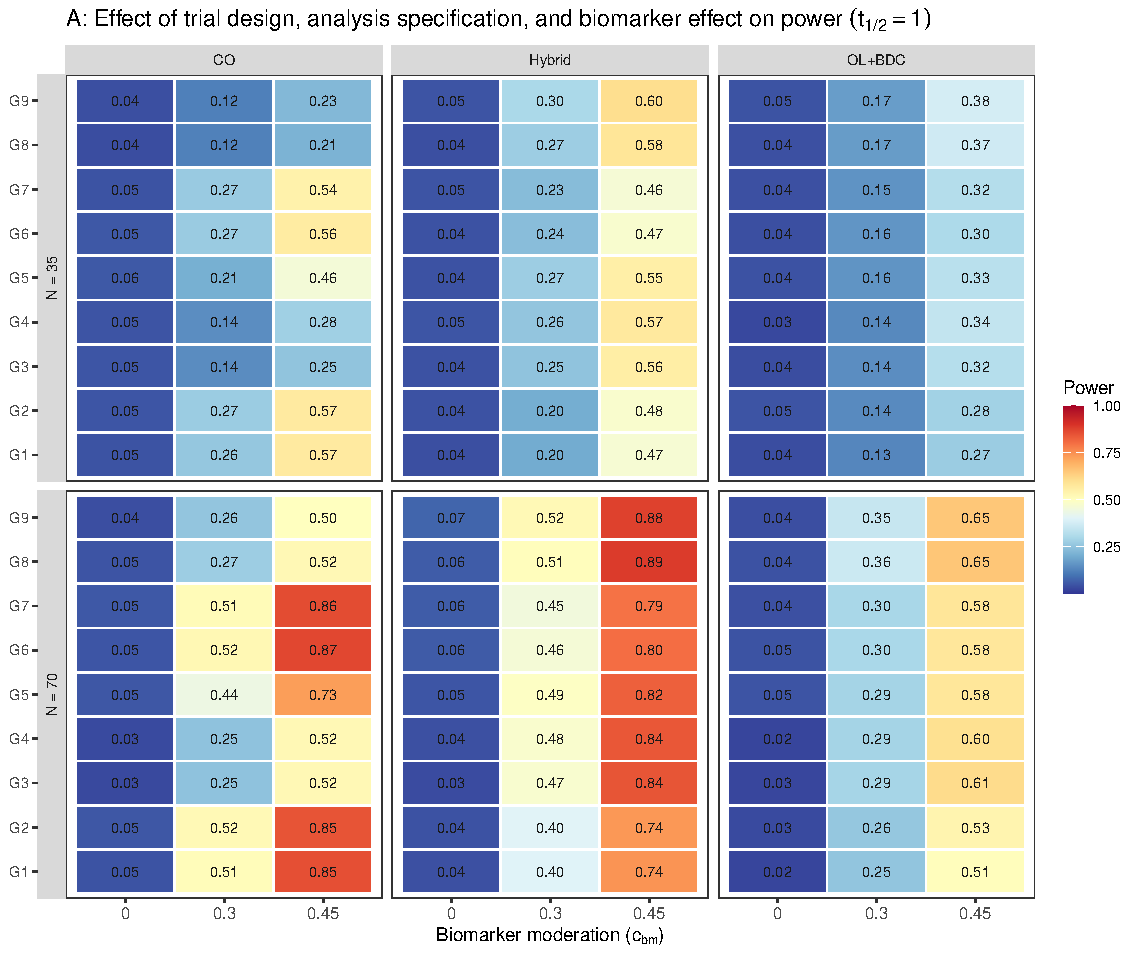
\includegraphics[width=0.95\linewidth]{../../figures/02xs-heatmap-hendrickson-a} \caption{Tier 1 grid, biomarker-effect axis: power by trial design (columns), $N$ (row blocks), and analysis specification (rows within block), across $c_{bm} \in \{0, 0.30, 0.45\}$ at $t_{1/2} = 1.0$ weeks, exponential DGP.}\label{fig:fig-hendrickson-a}
\end{figure}

\begin{figure}
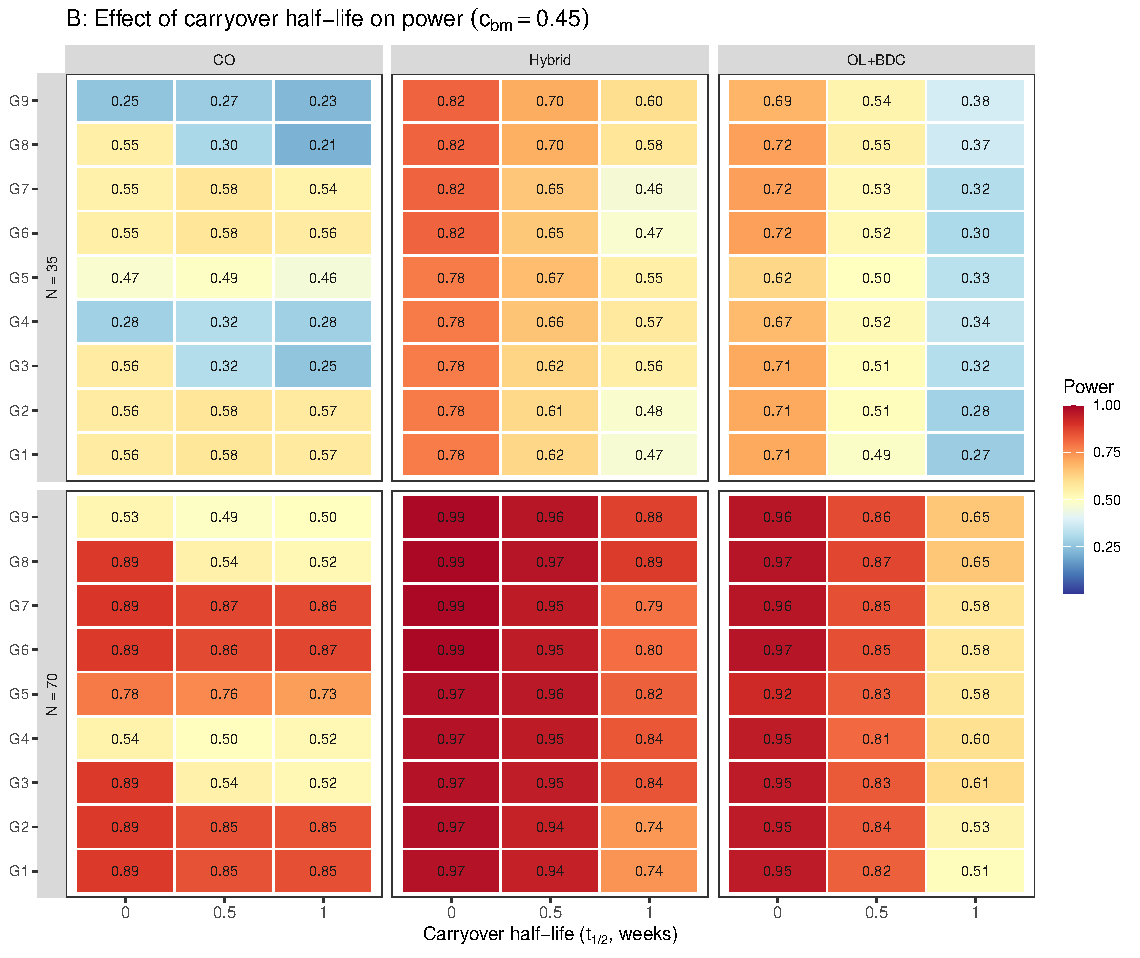
\includegraphics[width=0.95\linewidth]{../../figures/02xs-heatmap-hendrickson-b} \caption{Tier 1 grid, carryover-axis: power by trial design (columns), $N$ (row blocks), and analysis specification (rows within block), across $t_{1/2} \in \{0, 0.5, 1.0\}$ weeks at $c_{bm} = 0.45$, exponential DGP.}\label{fig:fig-hendrickson-b}
\end{figure}

\begin{figure}
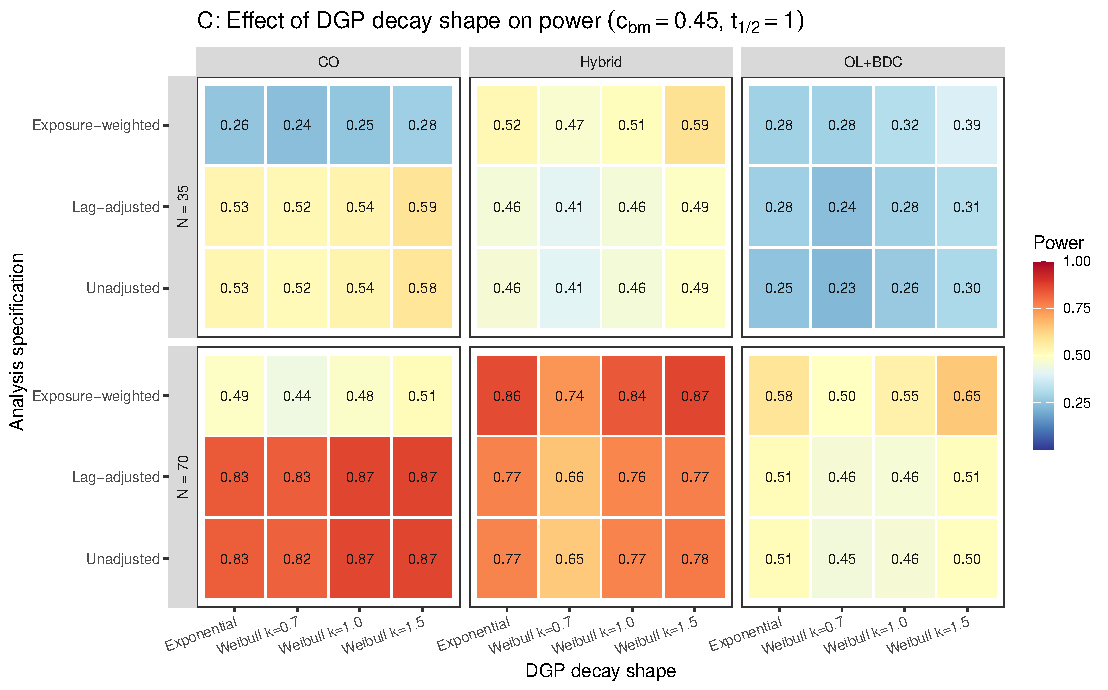
\includegraphics[width=0.95\linewidth]{../../figures/02xs-heatmap-hendrickson-c} \caption{Tier 1 grid, decay-shape axis: power by trial design (columns), $N$ (row blocks), and analysis specification (rows within block), across the four DGP decay-shape levels (exponential, Weibull $k \in \{0.7, 1.0, 1.5\}$) at $c_{bm} = 0.45$, $t_{1/2} = 1.0$ weeks. This axis has no Hendrickson analogue, whose grid used one decay form.}\label{fig:fig-hendrickson-c}
\end{figure}

Three features are visible at a glance that the headline table and
line plots elsewhere in this section make only cell-by-cell. First,
within every design x \(N\) block, the Unadjusted and Lag-adjusted
rows are numerically identical to two decimal places at every
biomarker level, half-life, and decay shape, the clean null of
Section 3.3 displayed across the entire grid at once rather than at
one reference cell. Second, the Exposure-weighted row visibly
separates from the other two only in the Hybrid and OL+BDC columns,
and only once carryover is present (Figure \ref{fig:fig-hendrickson-b});
in the CO column it is weaker than the other two at every half-life
past zero, the design-dependence of Section 3.4 read directly off
the grid. Third, Figure \ref{fig:fig-hendrickson-c} shows the
Exposure-weighted row's advantage in the Hybrid and OL+BDC columns
holding across every decay shape examined, including the
heaviest-tailed Weibull form (\(k = 0.7\)), the decay-form robustness
of Section 3.5 shown across the full grid rather than at one cell.

\subsection{Matched-decay baseline}\label{matched-decay-baseline}

At the matched cell (exponential DGP, exposure-weighted analysis,
\(N = 70\), \(c_{bm} = 0.45\), Hybrid design), power
declines from \(0.988 \pm 0.005\) at \(t_{1/2} = 0\) to
\(0.948 \pm 0.010\) at \(t_{1/2} = 0.5\) to \(0.860 \pm 0.016\) at
\(t_{1/2} = 1.0\) weeks (point estimate plus or minus MCSE,
\(n_{sim} = 500\)). All 500 replicates converged at every half-life in
this cell.

We had previously read the value at \(t_{1/2} = 1.0\) as agreeing with
the power of 0.82 reported by Hendrickson et al.~for a comparable
cell\textsuperscript{\citeproc{ref-hendrickson2020}{2}}. Unfortunately, we must withdraw that
comparison. In the
reference implementation, the analysis-side and data-generating
carryover parameters are set independently, and the drivers that
reproduce the original figures supply a half-life to the
data-generating step only, leaving the analysis-side half-life at
its default of zero, at which the exposure-decayed predictor
collapses onto the binary on-drug indicator. The reference analysis
is therefore Unadjusted, not Exposure-weighted, so the appropriate
comparator is our unadjusted power at the same cell, \(0.766\), and
the grids differ further on interaction strength and half-life, so
``the same cell'' was approximate in any case. We have not resolved
what the published figure was computed under, and make no claim of
agreement or disagreement here. Nothing else in this manuscript
depends on that comparison, since the three specifications are
compared against one another within a single simulation under common
random numbers.

\subsection{Power by analysis specification}\label{power-by-analysis-specification}

\begin{figure}
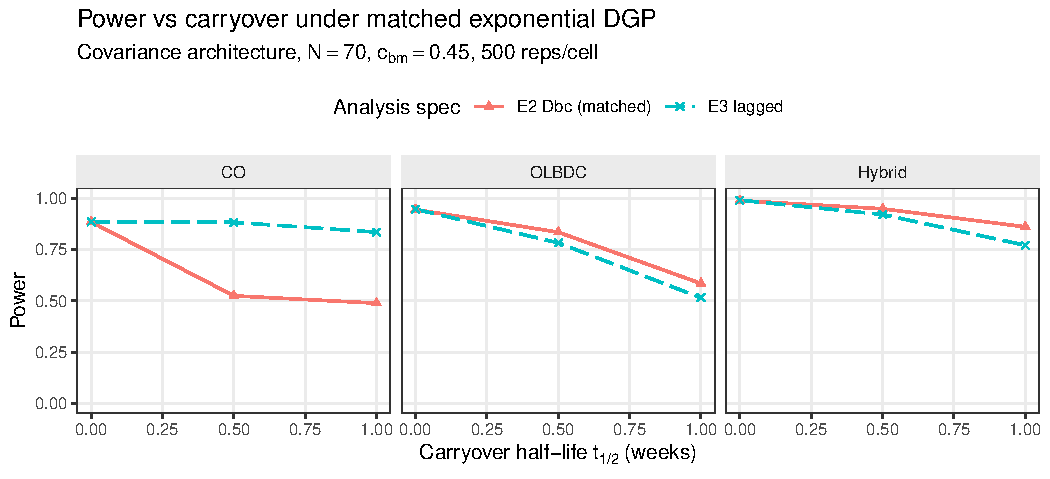
\includegraphics[width=0.95\linewidth]{../../figures/02xs-power-by-spec} \caption{Power versus carryover half-life under the exponential DGP, by analysis specification and trial design.}\label{fig:fig-power-by-spec}
\end{figure}

Two features of Figure \ref{fig:fig-power-by-spec} carry the
substance of this study. First, the Unadjusted and Lag-adjusted
curves lie on top of one another in every panel and at every
half-life. At the reference cell they give \(0.766\) and \(0.770\) at
\(t_{1/2} = 1.0\) weeks, and across all 216 cells the mean difference
is 0.003, with mean bias, MSE, and coverage agreeing to three
decimal places. Since the two share an estimand, are fitted to the
same simulated datasets, and differ by exactly one nuisance term,
this is as clean a null as the design can produce. The
lagged-treatment term contributes nothing on any measure (Section
4.1). Second, the three specifications give nearly identical power
at \(t_{1/2} = 0\), where there is no carryover to model, and diverge
as the half-life increases, with Exposure-weighted separating from
the other two. It retains a modest but consistent advantage in the
Hybrid and OL+BDC designs from \(t_{1/2} = 0.5\) weeks onward, but not
under the crossover design, where it is markedly inferior to both
alternatives (\(0.488\) against \(0.830\) for Unadjusted). This appears
to be because the within-subject correlation in a crossover trial
already carries most of the signal the decaying predictor targets,
so it gains little while its down-weighting of off-drug observations
works against it (Section 4).

\subsection{Decay-form mis-specification}\label{decay-form-mis-specification}

\begin{figure}
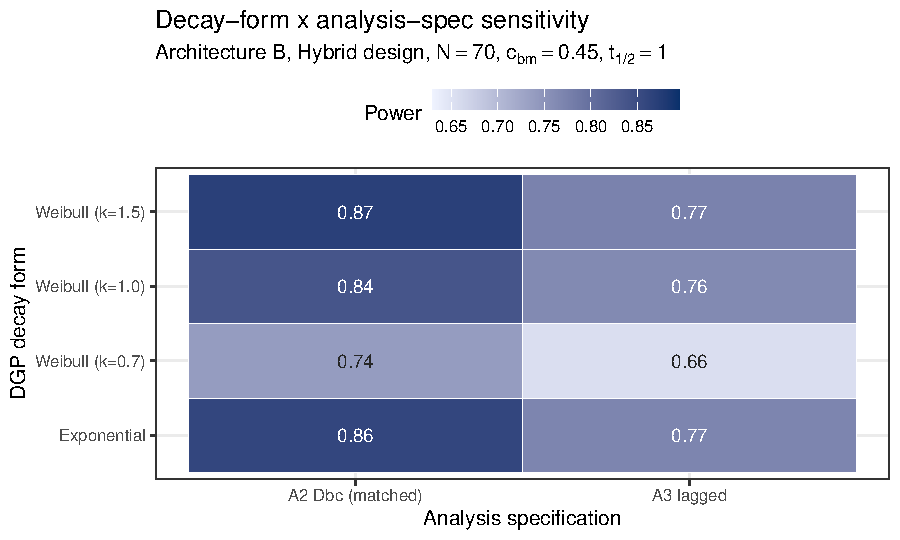
\includegraphics[width=0.78\linewidth]{../../figures/02xs-heatmap-matched-vs-mismatched} \caption{Power at the critical cell ($t_{1/2} = 1.0$ weeks, Hybrid, $N = 70$, $c_{bm} = 0.45$) across DGP decay forms (rows) and specifications (columns). Fill scale is stretched to the observed range, not [0,1], and not comparable to other figures.}\label{fig:fig-heatmap-mismatch}
\end{figure}

The heatmap cell at the intersection of the exponential DGP row and
the Exposure-weighted column is the matched reference, with power
\(0.860 \pm 0.016\). The Unadjusted and Lag-adjusted columns, invariant
to the assumed decay form by construction, are near-identical
throughout, as in Figure \ref{fig:fig-power-by-spec}, so variation
down those columns is data-generating decay and Monte Carlo noise.
The remaining Exposure-weighted rows give the cost of assuming
exponential decay when the truth is Weibull. Even at the
heaviest-tailed form examined (\(k = 0.7\)), its advantage narrows but
does not reverse (Section 4).

\subsection{Type I error control and cluster-robust recalibration}\label{type-i-error-control-and-cluster-robust-recalibration}

\begin{figure}
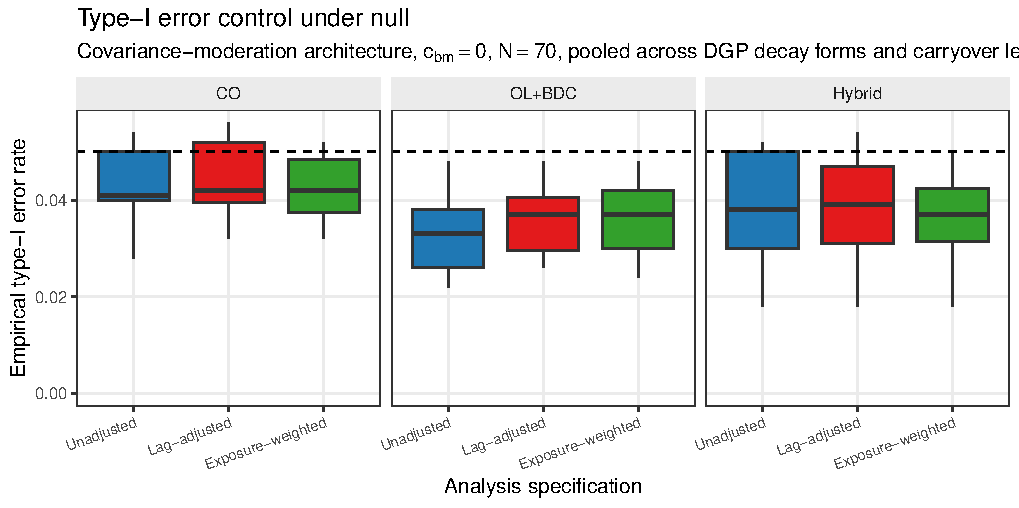
\includegraphics[width=0.8\linewidth]{../../figures/02xs-type1-boxplots} \caption{Empirical Type I error under the null, pooled across decay forms and half-lives, by design and specification ($N=70$, dashed line marks nominal 0.05).}\label{fig:fig-type1}
\end{figure}

Across the null cells, empirical Type I error sits uniformly below
the nominal 0.05 level for all three specifications and designs
(design-level means 0.032 to 0.041). This is not sampling noise but
the conservatism of the model-based test (Section 2.6), from a
working covariance that does not match the data-generating one.
Because the conservatism is uniform across specifications, it does
not disturb the comparison among them, and the block S6
recalibration below confirms that a CR2 cluster-robust standard
error restores nominal rejection without changing which
specification leads. This also establishes that the null result of
Section 3.3 is not an artifact of differential test size, since
Unadjusted and Lag-adjusted are conservative to the same degree.
Table \ref{tab:tab-type1-cr2} makes this explicit at the null
cell.

\begin{table}

\caption{\label{tab:tab-type1-cr2}Conservatism of the model-based interaction test and its
    cluster-robust correction, at the null cell ($c_{bm} = 0$,
    exponential DGP, $t_{1/2} = 1.0$ weeks, Hybrid design, $N = 70$,
    3{,}000 replicates).
    $\kappa$ is the calibration ratio defined in Section 2.6.
    $\kappa > 1$ indicates a conservative
    test. All three specifications are conservative under the
    model-based test, most so Exposure-weighted ($\kappa = 1.10$,
    Type I $= 0.029$). The CR2 bias-reduced cluster-robust standard
    error restores $\kappa$ to near one and Type I to nominal (0.045
    to 0.049) for all three.}
\centering
\begin{tabular}[t]{lllll}
\toprule
Specification & $\kappa$ model & Type I model & $\kappa$ CR2 & Type I CR2\\
\midrule
Unadjusted & 1.06 & 0.036 & 0.98 & 0.048\\
Lag-adjusted & 1.05 & 0.039 & 0.98 & 0.049\\
Exposure-weighted & 1.10 & 0.029 & 1.00 & 0.045\\
\bottomrule
\end{tabular}
\end{table}

\begin{table}
\centering
\caption{\label{tab:tab-s6}Cluster-robust recalibration at the reference cell and
    four stress cells (500 replicates, $c_{bm} = 0.45$). EW is
    Exposure-weighted,
    LA is Lag-adjusted, U is Unadjusted. $\kappa$ is the calibration
    ratio of Section 2.6, here for Exposure-weighted. A value above
    one is a
    conservative test. The two gap pairs give each alternative
    against the unadjusted benchmark under each inference. CR2 df is
    the mean Satterthwaite degrees of freedom for the cluster-robust
    test on Exposure-weighted. Computed with
    \texttt{clubSandwich}.}
\centering
\resizebox{\ifdim\width>\linewidth\linewidth\else\width\fi}{!}{
\begin{tabular}[t]{llllllllll}
\toprule
Cell & $\kappa$ model & $\kappa$ CR2 & EW model & EW CR2 & EW$-$U model & EW$-$U CR2 & LA$-$U model & LA$-$U CR2 & CR2 df\\
\midrule
Reference, $N=70$ & 1.15 & 0.99 & 0.829 & 0.863 & +0.080 & +0.092 & -0.003 & +0.002 & 23\\
Small $N=35$ & 1.13 & 0.96 & 0.558 & 0.590 & +0.066 & +0.086 & -0.002 & +0.000 & 12\\
High autocorr, $\rho=0.9$ & 1.26 & 0.94 & 0.954 & 0.980 & +0.052 & +0.032 & +0.000 & -0.004 & 23\\
Half-life mis-spec & 1.14 & 1.00 & 0.759 & 0.795 & +0.010 & +0.024 & -0.003 & +0.002 & 23\\
30\% MCAR dropout & 0.99 & 0.85 & 0.148 & 0.126 & +0.010 & +0.010 & -0.004 & +0.010 & 5\\
\bottomrule
\end{tabular}}
\end{table}

\begin{figure}
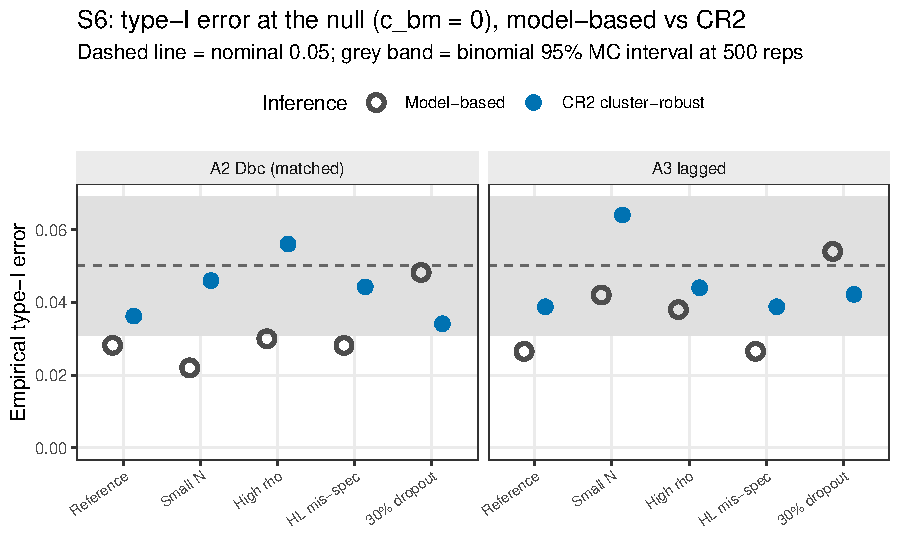
\includegraphics[width=0.95\linewidth]{../../figures/02xs-type1-cr2} \caption{Empirical Type I error at the null ($c_{bm} = 0$) under model-based and CR2 cluster-robust inference, across the five S6 stress cells and the three specifications. The model-based test (open) is conservative (near 0.03), and CR2 (filled) is restored to the nominal 0.05 (dashed), within the binomial Monte Carlo band (gray). 500 null replicates per cell.}\label{fig:fig-type1-cr2}
\end{figure}

Figure \ref{fig:fig-type1-cr2} confirms this directly. The
model-based rejection rate sits below nominal across all five S6
cells and all three specifications, while CR2 restores it to within
the Monte Carlo band around 0.05, and in the information-rich cells
the calibration ratio \(\kappa\) runs from 1.07 to 1.26 under the
model-based test, restored to about one under CR2, recovering two to
five points of power. Table \ref{tab:tab-s6} reports both
alternatives against the unadjusted benchmark. The Exposure-weighted
advantage is held or slightly widened under CR2 at the reference
cell (\(+0.080\) to \(+0.092\)), the small-\(N\) cell (\(+0.066\) to
\(+0.086\)), and the half-life mis-specification cell (\(+0.010\) to
\(+0.024\)). It narrows under high autocorrelation (\(+0.052\) to
\(+0.032\), though it still leads), and is small under 30\% MCAR
dropout (\(+0.010\)), which we read as the S3 finding restated, since
dropout removes the off-drug information the advantage depends on.
The Lag-adjusted gap, by contrast, is within \(\pm 0.010\) of zero at
every cell under either inference, corroborating the Section 3.3
null under a second procedure and at four stress cells the main grid
does not cover. This recalibration was validated only in the Hybrid,
\(N = 70\) cells, and should not be extended to the crossover design,
where Exposure-weighted does not lead in the first place.

\subsection{Sensitivity analyses}\label{sensitivity-analyses}

Seven Tier 2 blocks (S1-S4, S7, S8, S9) perturb one axis at a time
around a common reference cell (Hybrid, \(N = 70\), \(c_{bm} = 0.45\),
exponential DGP, \(t_{1/2} = 1.0\)), holding the remaining factors
fixed, except S9, which changes the trial design itself; an eighth,
S6, applies the cluster-robust correction of Section 3.5 at that
same cell plus four stress cells, and a ninth, S5, is exploratory
and reported only in the archived full-scope drafts. The blocks are
reported separately here and are not pooled with Tier 1 or with
each other.

\subsubsection{S1: within-factor autocorrelation}\label{s1-within-factor-autocorrelation}

\begin{figure}
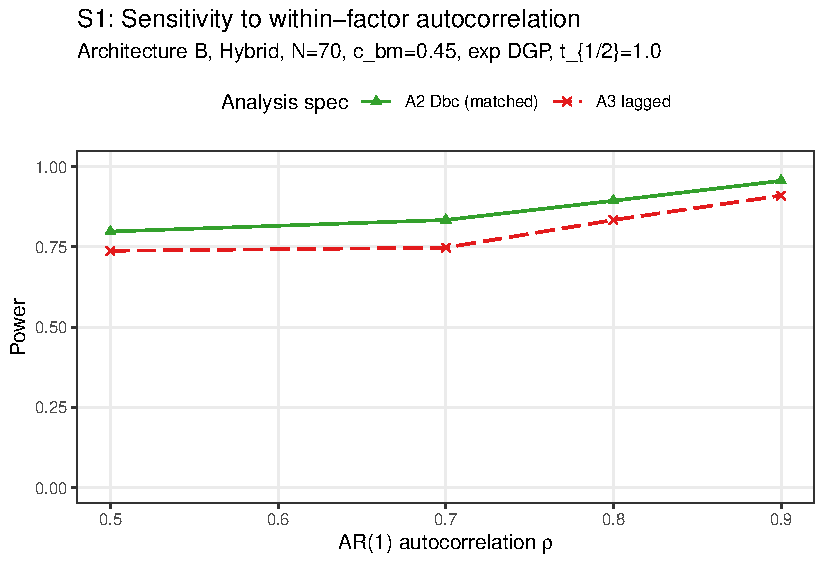
\includegraphics[width=0.6\linewidth]{../../figures/02xs-sens-S1} \caption{Power by analysis specification across AR(1) autocorrelation $\rho \in \{0.5, 0.7, 0.8, 0.9\}$.}\label{fig:fig-sens-s1}
\end{figure}

\begin{figure}
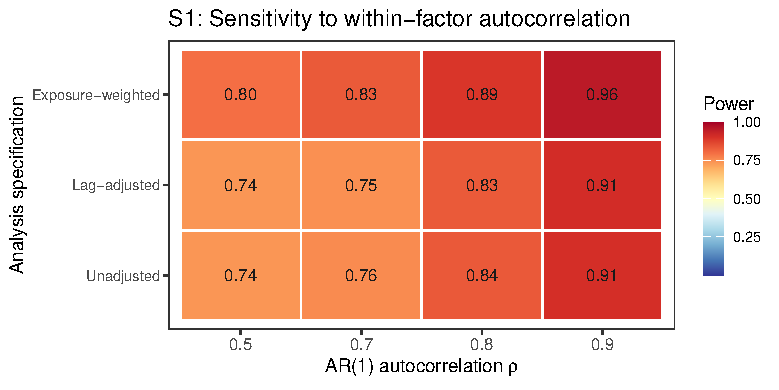
\includegraphics[width=0.7\linewidth]{../../figures/02xs-heatmap-sens-S1} \caption{Block S1 as a Hendrickson-style annotated heatmap: same data as Figure \\ref{fig:fig-sens-s1}.}\label{fig:fig-heatmap-sens-s1}
\end{figure}

All three specifications gain power monotonically with \(\rho\), from
\(0.798 \pm 0.018\) (Exposure-weighted) and \(0.738 \pm 0.020\) (the
other two, identical to three decimals) at \(\rho = 0.5\), to
\(0.956 \pm 0.009\) against \(0.906\) to \(0.910\) at \(\rho = 0.9\). The
Exposure-weighted advantage, roughly 0.05 to 0.08 in absolute power,
is preserved at every autocorrelation level examined, suggesting
autocorrelation strength and specification choice act additively
rather than interacting. Lag-adjusted tracks Unadjusted throughout,
never differing by more than 0.008.

\subsubsection{S2: analyst-truth half-life mismatch}\label{s2-analyst-truth-half-life-mismatch}

\begin{figure}
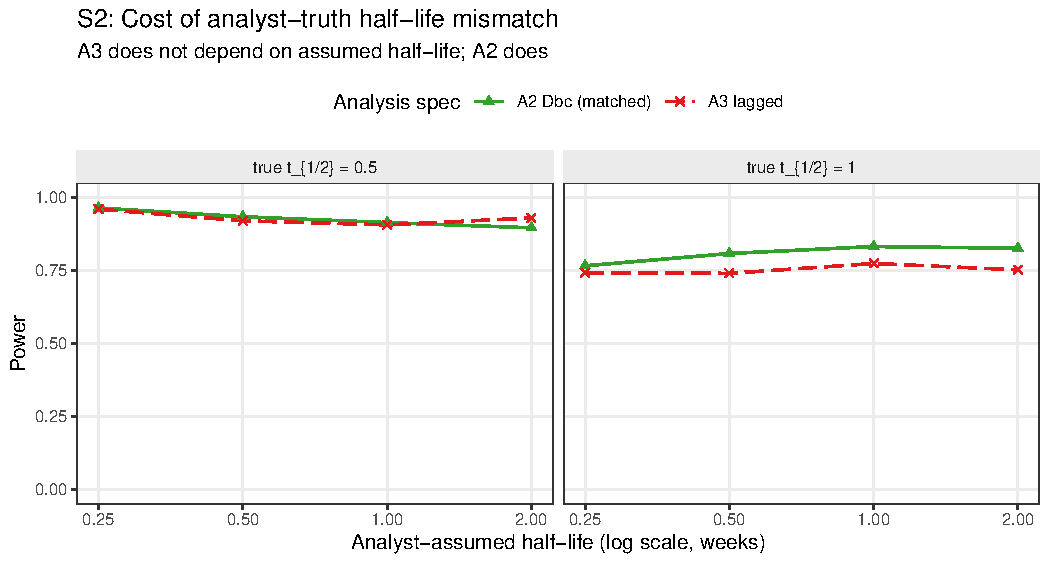
\includegraphics[width=0.8\linewidth]{../../figures/02xs-sens-S2} \caption{Power as the analyst's assumed half-life departs from the true DGP half-life. Only Exposure-weighted consumes the assumed half-life. Unadjusted and Lag-adjusted are invariant to it by construction and appear as flat reference lines.}\label{fig:fig-sens-s2}
\end{figure}

\begin{figure}
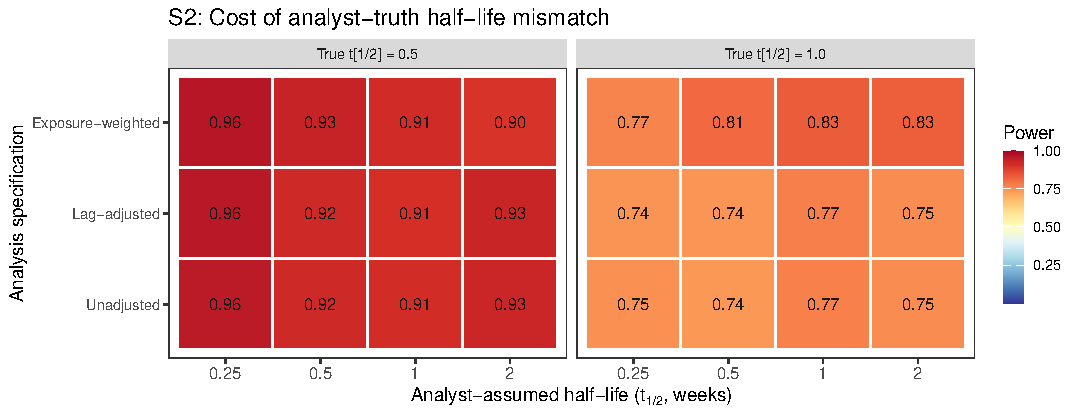
\includegraphics[width=0.9\linewidth]{../../figures/02xs-heatmap-sens-S2} \caption{Block S2 as a Hendrickson-style annotated heatmap: same data as Figure \\ref{fig:fig-sens-s2}, faceted by true half-life.}\label{fig:fig-heatmap-sens-s2}
\end{figure}

Block S2 crosses two true half-lives (\(t_{1/2} \in \{0.5, 1.0\}\)
weeks) with four analyst-assumed values (\(\hat{t}_{1/2} \in \{0.25,
0.5, 1.0, 2.0\}\) weeks), giving eight cells. Only Exposure-weighted
consumes \(\hat{t}_{1/2}\), so the cost of a wrong assumption must be
read within a true half-life rather than pooled across the block.

The penalty is modest. At a true half-life of 1.0 weeks,
Exposure-weighted attains 0.832 correctly specified, versus 0.766,
0.808, and 0.826 at assumed values of 0.25, 0.5, and 2.0 weeks. The
worst case, a fourfold under-assumption, costs 6.6 points and still
leaves it above both alternatives (0.746, 0.742). At a true
half-life of 0.5 weeks it attains 0.934 correctly specified, against
0.964, 0.914, and 0.896 at the same four assumed values. Because
Unadjusted and Lag-adjusted cannot depend on \(\hat{t}_{1/2}\), their
variation along that axis is pure Monte Carlo error, ranging 0.910
to 0.960 at a true half-life of 0.5 weeks. This roughly four- to
five-point noise floor explains the apparent anomaly that assuming
0.25 weeks (0.964) beats correct specification (0.934), a difference
well inside it. It also qualifies the one case where the direction
is worth noting. At a true half-life of 0.5 weeks with an assumed
value of 2.0 weeks, Exposure-weighted falls to 0.896, below both
alternatives (0.926, 0.930), so a fourfold over-assumption erodes
its advantage to a tie.

The practical reading is that an approximate half-life is adequate,
with an asymmetry. Under-assuming is safer than over-assuming. This
follows from the limiting-case relationship of Section 2.4, since
shrinking \(\hat{t}_{1/2}\) drives the predictor toward the binary
indicator, which remains serviceable, whereas inflating it drives
the predictor toward a constant, at which the on-off contrast and
the estimand itself degenerate.

\subsubsection{S3: dropout}\label{s3-dropout}

\begin{figure}
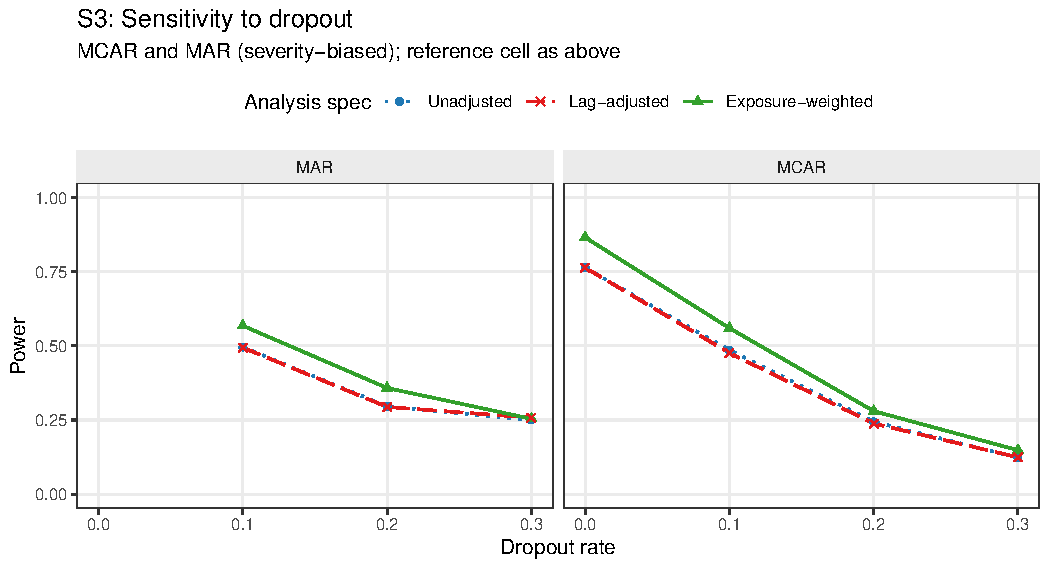
\includegraphics[width=0.8\linewidth]{../../figures/02xs-sens-S3} \caption{Power at dropout rates $\in \{0, 0.1, 0.2, 0.3\}$ under MCAR and MAR mechanisms.}\label{fig:fig-sens-s3}
\end{figure}

\begin{figure}
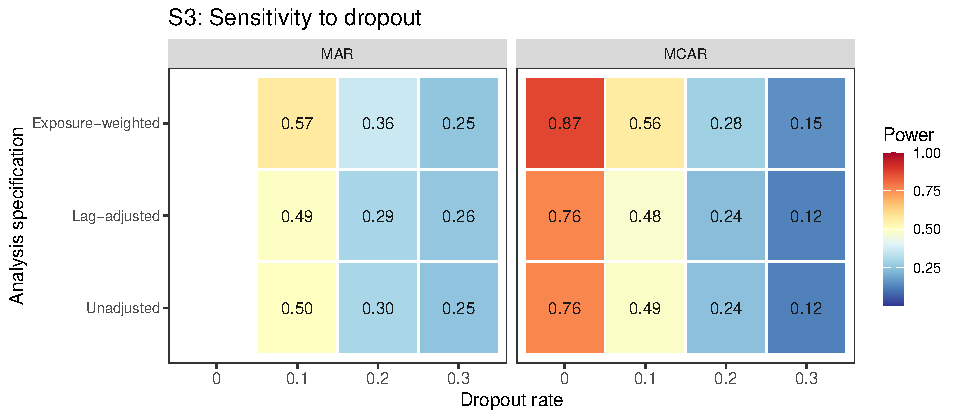
\includegraphics[width=0.8\linewidth]{../../figures/02xs-heatmap-sens-S3} \caption{Block S3 as a Hendrickson-style annotated heatmap: same data as Figure \\ref{fig:fig-sens-s3}, faceted by dropout mechanism. The MAR arm has no $0\%$ cell (Section 3.6); it shares the MCAR reference cell.}\label{fig:fig-heatmap-sens-s3}
\end{figure}

All three specifications lose power monotonically as dropout
increases. At the MCAR baseline (\(N = 70\), no dropout),
Exposure-weighted gives \(0.866 \pm 0.015\) against \(0.764 \pm 0.019\)
for the other two. At 30\% MCAR dropout, all three collapse to
\(0.122\) to \(0.148\). The Exposure-weighted advantage narrows steadily
as dropout worsens, from about 0.10 absolute at zero dropout to 0.07
at 10\%, 0.04 at 20\%, and 0.03 at 30\% under MCAR, narrowing further
under MAR at the highest rate. This is consistent with the advantage
originating in the exposure-weighted contrast from off-drug
observations, which contracts as those observations are
preferentially lost. The advantage is preserved at dropout of 20\% or
below. Lag-adjusted again tracks Unadjusted throughout, the largest
discrepancy being 0.010.

\subsubsection{S4: biomarker-moderation effect-size curve}\label{s4-biomarker-moderation-effect-size-curve}

\begin{figure}
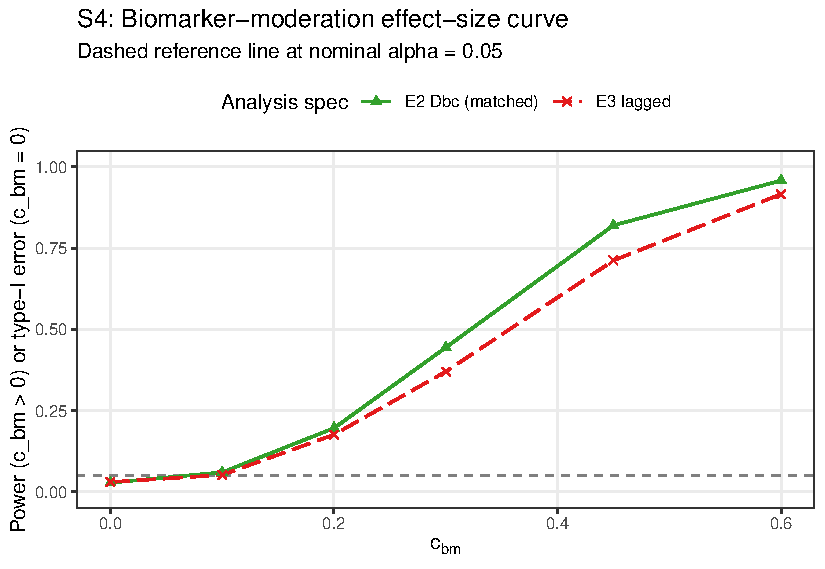
\includegraphics[width=0.6\linewidth]{../../figures/02xs-sens-S4} \caption{Power across the biomarker-moderation effect-size range $c_{bm} \in \{0, 0.10, 0.20, 0.30, 0.45, 0.60\}$. The $c_{bm} = 0$ point is the null for Type I verification.}\label{fig:fig-sens-s4}
\end{figure}

\begin{figure}
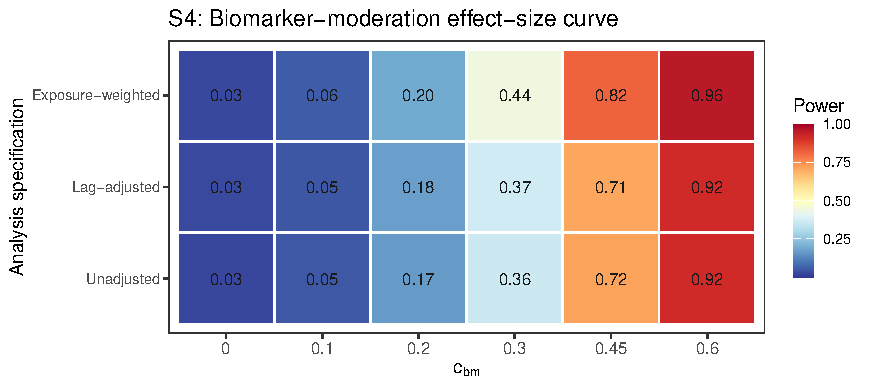
\includegraphics[width=0.7\linewidth]{../../figures/02xs-heatmap-sens-S4} \caption{Block S4 as a Hendrickson-style annotated heatmap: same data as Figure \\ref{fig:fig-sens-s4}.}\label{fig:fig-heatmap-sens-s4}
\end{figure}

The power curve is sigmoidal for all three specifications. At
\(c_{bm} = 0\), empirical Type I error sits below nominal for each
(0.026 to 0.030). Power then rises through the mid-range and
saturates once \(c_{bm} \geq 0.45\), reaching 0.916 to 0.958 at
\(c_{bm} = 0.6\). The Exposure-weighted advantage over the unadjusted
benchmark is largest at intermediate effect sizes, \(+0.082\) absolute
at \(c_{bm} = 0.30\) and \(+0.102\) at \(c_{bm} = 0.45\), shrinking to
\(+0.042\) at \(c_{bm} = 0.60\) as all three approach the ceiling, so
the advantage matters most for trials targeting a moderate
biomarker-treatment interaction. Lag-adjusted and Unadjusted
coincide across the entire range, differing by at most 0.008.

\subsubsection{S7: biomarker-interacted carryover terms}\label{s7-biomarker-interacted-carryover-terms}

Every carryover term evaluated so far, Lag-adjusted (Section 2.4)
and the exploratory washout-adjusted check of Section 4.1, enters
the model as a nuisance main effect only, so by construction neither
can repair the attenuated \(\text{bm:}D_{it}\) coefficient (Section
1). Here we test the two elaborations Section 4.6 identifies as the
natural next step: crossing the same lagged and washout carryover
terms with \(bm\), so the biomarker effect itself is allowed to
decline across the washout rather than committing to a rate, \texttt{E5}
(\(\text{Sx} \sim bm + t + D_{it} + \text{bm:}D_{it} + L_{it} +
\text{bm:}L_{it}\)) and \texttt{E6} (\(\text{Sx} \sim bm + t + D_{it} +
\text{bm:}D_{it} + t_{sd} + \text{bm:}t_{sd}\)). Because these add a
second interaction coefficient, the interaction test is not the same
single-coefficient Wald statistic used elsewhere. We report the
joint 2-df Wald test of \(\text{bm:}D_{it}\) and the second coefficient
together (\texttt{nlme::anova.lme(Terms\ =\ ...)}), the only test that
reflects whether coupling the biomarker to the carryover term
recovers power, against Unadjusted and the washout main-effect check
(\texttt{E4}) as single-coefficient benchmarks.

\begin{table}
\centering
\caption{\label{tab:tab-s7}Block S7: biomarker-interacted carryover terms at the
    reference cell (Hybrid, $N = 70$, $c_{bm} = 0.45$,
    $t_{1/2} = 1.0$, exponential DGP, $n_{sim} = 500$, all
    replicates converged). Power for E5/E6 is the joint 2-df Wald
    test of bm:Db and the second interaction coefficient together;
    power for E1/E4 is the usual single-coefficient test. Mean bm:Db
    is the average point estimate of the bm:Db coefficient alone in
    each fitted model (comparable in form, not necessarily in
    calibration, across rows). The last column is the rejection
    rate of the bm:Db coefficient tested by itself, ignoring the
    second term, shown as a diagnostic only.}
\centering
\resizebox{\ifdim\width>\linewidth\linewidth\else\width\fi}{!}{
\begin{tabular}[t]{lllll}
\toprule
Specification & Test & Power (MCSE) & Mean bm:Db & bm:Db alone, reject.\ rate\\
\midrule
Unadjusted & Single-coef. & 0.748 (0.019) & -2.392 & 0.748\\
Washout main effect & Single-coef. & 0.750 (0.019) & -2.394 & 0.750\\
Lag $\times$ bm & Joint (2 df) & 0.690 (0.021) & -2.990 & 0.720\\
Washout $\times$ bm & Joint (2 df) & 0.704 (0.020) & -1.561 & 0.198\\
\bottomrule
\end{tabular}}
\end{table}

\begin{figure}
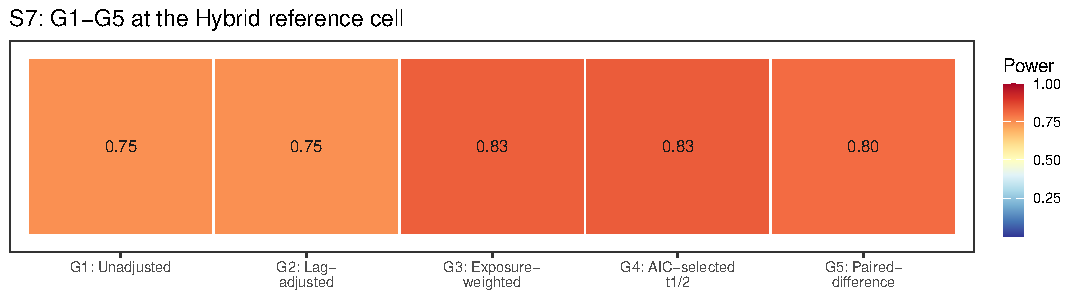
\includegraphics[width=0.75\linewidth]{../../figures/02xs-heatmap-sens-S7} \caption{Block S7 as a Hendrickson-style annotated heatmap: same power figures as Table \\ref{tab:tab-s7}, E5/E6 columns are the joint 2-df test.}\label{fig:fig-heatmap-sens-s7}
\end{figure}

Table \ref{tab:tab-s7} gives a clean negative result. Both
interacted specifications have \emph{lower} joint-test power than the
unadjusted benchmark, \texttt{E5} by 5.8 points and \texttt{E6} by 4.4 points,
despite each visibly moving the \(\text{bm:}D_{it}\) point estimate
relative to \texttt{E1}. \texttt{E5}'s estimate is less attenuated on average
(\(-2.990\) against \(-2.392\) for \texttt{E1}), consistent with the lagged
interaction term absorbing some of the attenuation as intended, but
the extra degree of freedom the joint test spends is not informative
enough to turn that into a net power gain. \texttt{E6} is worse: its
\(\text{bm:}D_{it}\) estimate is pulled toward zero (\(-1.561\)) and its
single-coefficient rejection rate collapses to \(0.198\) from \texttt{E1}'s
\(0.748\), evidence of severe coefficient instability from
collinearity between \(\text{bm:}D_{it}\) and \(\text{bm:}t_{sd}\), since
\(t_{sd}\) is a near-deterministic function of \(D_{it}\) and elapsed
time within this trial design. Interacting a carryover nuisance term
with the biomarker is a theoretically motivated fix for the
attenuation mechanism identified in Section 1, but at this reference
cell it does not recover power over the unadjusted benchmark under
either functional form, and the washout form additionally
destabilizes the very coefficient it was meant to unbias. This
closes the ``adjacent specification\ldots{} not evaluated'' gap raised in
Section 4.6, with a negative answer; it was checked at a single
reference cell only and should not be read as ruling out every
biomarker-interacted carryover term. Section 4.5 discusses what
would need to be true for a term like this to help.

\subsubsection{S8: architecture sensitivity of the specification ranking}\label{s8-architecture-sensitivity-of-the-specification-ranking}

Every result reported to this point, Tier 1 and blocks S1-S7 alike,
is restricted to Architecture B (covariance moderation), the
manuscript's stated scope (Section 2.3). Block S8 asks a narrower
question than a full architecture comparison, which is the purpose
of the companion manuscript on DGP architectures\textsuperscript{\citeproc{ref-pmsimstats_dgp_architectures2026}{3}}: does the ranking among analysis
specifications established above under Architecture B hold under
Architecture A (mean moderation) as well, or is the choice of
carryover representation itself architecture-dependent? We refit the
five specifications of block S7's table (\texttt{E1}, Lag-adjusted \texttt{E3},
Exposure-weighted \texttt{E2}, \texttt{E5}, \texttt{E6}) at the same reference cell under
both architectures, now at three half-lives (\(t_{1/2} \in \{0, 0.5,
1.0\}\)) rather than the single reference value, so the check covers
whether the ranking is architecture-dependent uniformly or only once
carryover is severe enough. Because \(c_{bm}\) is not calibrated to
equal power across architectures, the two produce materially
different absolute power at the same nominal value (Section 1;\textsuperscript{\citeproc{ref-pmsimstats_dgp_architectures2026}{3}} shows the mean-moderation channel
requires several times the nominal effect size for a comparable
power loss under carryover); only the within-architecture ranking is
the object of interest here.

\begin{table}
\centering
\caption{\label{tab:tab-s8}Block S8: analysis-specification ranking by DGP
    architecture and carryover half-life, at the reference cell
    (Hybrid, $N = 70$, $c_{bm} = 0.45$, exponential DGP,
    $n_{sim} = 500$). E5/E6 power is the joint 2-df Wald test as in
    Table \\ref{tab:tab-s7}. Absolute power is not comparable
    between architectures at the same nominal $c_{bm}$; only the
    within-architecture ranking is of interest.}
\centering
\resizebox{\ifdim\width>\linewidth\linewidth\else\width\fi}{!}{
\fontsize{9}{11}\selectfont
\begin{tabular}[t]{lrlll}
\toprule
Architecture & t1/2 & Specification & Power (MCSE) & Non-conv\\
\midrule
B (covariance) & 0.0 & Unadjusted & 0.982 (0.006) & 0.000\\
B (covariance) & 0.0 & Lag-adjusted & 0.980 (0.006) & 0.000\\
B (covariance) & 0.0 & Exposure-weighted & 0.982 (0.006) & 0.000\\
B (covariance) & 0.0 & Lag $\times$ bm & 0.940 (0.011) & 0.000\\
B (covariance) & 0.0 & Washout $\times$ bm & 0.944 (0.010) & 0.000\\
\addlinespace
B (covariance) & 0.5 & Unadjusted & 0.922 (0.012) & 0.000\\
B (covariance) & 0.5 & Lag-adjusted & 0.920 (0.012) & 0.000\\
B (covariance) & 0.5 & Exposure-weighted & 0.936 (0.011) & 0.000\\
B (covariance) & 0.5 & Lag $\times$ bm & 0.870 (0.015) & 0.000\\
B (covariance) & 0.5 & Washout $\times$ bm & 0.862 (0.015) & 0.000\\
\addlinespace
B (covariance) & 1.0 & Unadjusted & 0.760 (0.019) & 0.000\\
B (covariance) & 1.0 & Lag-adjusted & 0.760 (0.019) & 0.000\\
B (covariance) & 1.0 & Exposure-weighted & 0.836 (0.017) & 0.000\\
B (covariance) & 1.0 & Lag $\times$ bm & 0.688 (0.021) & 0.000\\
B (covariance) & 1.0 & Washout $\times$ bm & 0.714 (0.020) & 0.000\\
\addlinespace
A (mean) & 0.0 & Unadjusted & 0.972 (0.007) & 0.000\\
A (mean) & 0.0 & Lag-adjusted & 0.972 (0.007) & 0.000\\
A (mean) & 0.0 & Exposure-weighted & 0.972 (0.007) & 0.000\\
A (mean) & 0.0 & Lag $\times$ bm & 0.940 (0.011) & 0.000\\
A (mean) & 0.0 & Washout $\times$ bm & 0.928 (0.012) & 0.000\\
\addlinespace
A (mean) & 0.5 & Unadjusted & 0.968 (0.008) & 0.000\\
A (mean) & 0.5 & Lag-adjusted & 0.968 (0.008) & 0.000\\
A (mean) & 0.5 & Exposure-weighted & 0.966 (0.008) & 0.000\\
A (mean) & 0.5 & Lag $\times$ bm & 0.932 (0.011) & 0.000\\
A (mean) & 0.5 & Washout $\times$ bm & 0.930 (0.011) & 0.000\\
\addlinespace
A (mean) & 1.0 & Unadjusted & 0.972 (0.007) & 0.000\\
A (mean) & 1.0 & Lag-adjusted & 0.976 (0.007) & 0.000\\
A (mean) & 1.0 & Exposure-weighted & 0.946 (0.010) & 0.000\\
A (mean) & 1.0 & Lag $\times$ bm & 0.940 (0.011) & 0.000\\
A (mean) & 1.0 & Washout $\times$ bm & 0.940 (0.011) & 0.000\\
\bottomrule
\end{tabular}}
\end{table}

\begin{figure}
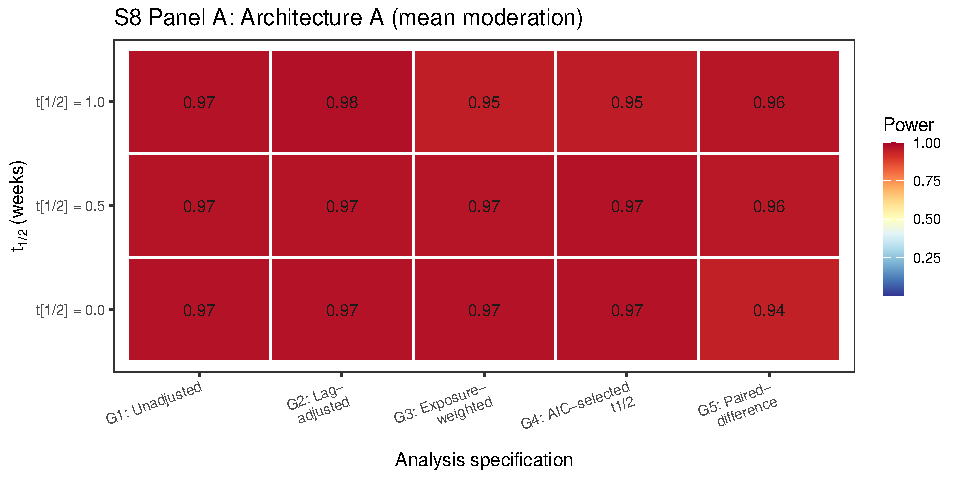
\includegraphics[width=0.8\linewidth]{../../figures/02xs-heatmap-sens-S8-a} \caption{Block S8, Panel A (Architecture A, mean moderation): power by carryover half-life (rows) and analysis specification (columns). Same data as the Architecture A rows of Table \\ref{tab:tab-s8}.}\label{fig:fig-heatmap-sens-s8a}
\end{figure}

\begin{figure}
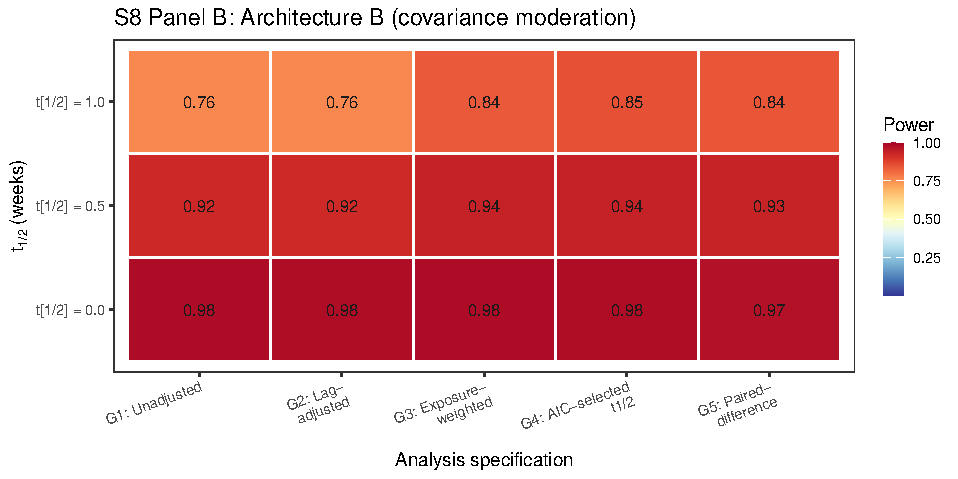
\includegraphics[width=0.8\linewidth]{../../figures/02xs-heatmap-sens-S8-b} \caption{Block S8, Panel B (Architecture B, covariance moderation): power by carryover half-life (rows) and analysis specification (columns). Same data as the Architecture B rows of Table \\ref{tab:tab-s8}. Not directly comparable to Panel A in absolute terms (Section 3.6).}\label{fig:fig-heatmap-sens-s8b}
\end{figure}

Table \ref{tab:tab-s8} and Figures \ref{fig:fig-heatmap-sens-s8a}/
\ref{fig:fig-heatmap-sens-s8b} show the ranking is architecture-dependent
for exactly one specification, and the dependence grows with
carryover severity rather than switching on at some threshold. At
\(t_{1/2} = 0\) every specification collapses to the same estimand in
both architectures (no carryover to represent), so Unadjusted and
Exposure-weighted agree there by construction in each panel (both
\(0.982\) under B, both \(0.972\) under A). Under Architecture B,
Exposure-weighted overtakes Unadjusted by \(t_{1/2} = 0.5\) (\(0.936\)
versus \(0.922\), a 1.4-point edge) and leads clearly by \(t_{1/2} = 1.0\)
(\(0.836\) versus \(0.760\), an 7.6-point edge). Under Architecture A the
pattern reverses in sign at both nonzero half-lives, though the
magnitude stays small: Exposure-weighted trails by 0.2 points at
\(t_{1/2} = 0.5\) (\(0.966\) versus \(0.968\)) and by 2.6 points at
\(t_{1/2} = 1.0\) (\(0.946\) versus \(0.972\)), the latter about 1.5 MCSE
and so a real, if modest, reversal rather than pure noise. This
matches the pattern already reported from the full-scope grid in the
archived drafts, that Exposure-weighted is marginally dominated in
every design examined under mean moderation (Section 4.6), now
confirmed directly within this manuscript across the half-life range
rather than at one value alone. Lag-adjusted (\texttt{E3}) remains
statistically indistinguishable from Unadjusted (\texttt{E1}) under both
architectures at every half-life (largest gap 0.004, well under one
MCSE), extending Section 3.3's clean null to Architecture A as well.
The S7 negative result also replicates here: \texttt{E5} and \texttt{E6} sit below
the \texttt{E1}/\texttt{E3} benchmark under both architectures at every half-life
examined, including \(t_{1/2} = 0\), where the extra degree of freedom
still costs power even with no true carryover to model, so
biomarker-interacted carryover terms recover power in neither
architecture nor at any carryover severity tested. The one
specification recommendation this manuscript makes, exposure
weighting in the Hybrid and OL+BDC designs (Conclusions), is
therefore itself conditional on Architecture B and grows more
important as carryover worsens; this check confirms that restriction
across the half-life range rather than at one cell,
and the recommendation should not be extrapolated to Architecture A,
where the archived full-scope drafts remain the authority.

\subsubsection{S9: does a longer, graded washout help the biomarker-interacted terms?}\label{s9-does-a-longer-graded-washout-help-the-biomarker-interacted-terms}

Block S7 (Section 3.6) found the two biomarker-interacted carryover
specifications, \texttt{E5} and \texttt{E6}, underperform the unadjusted benchmark
at the Hybrid reference cell, and traced part of the reason to a
design artifact: \texttt{E6}'s \(\text{bm:}t_{sd}\) coefficient is
collinear with \(\text{bm:}D_{it}\) because \(t_{sd}\) barely varies
across Hybrid's one- to two-occasion off-drug window (Section 4.5).
The CO design's off-drug arm instead runs from 2.5 to 20 weeks
post-discontinuation (Section 2.2), a far more graded range of
\(t_{sd}\) values. Block S9 asks whether refitting \texttt{E1}, \texttt{E4}, \texttt{E5},
and \texttt{E6} under CO, at two true half-lives, lets the interacted
specifications close the gap.

\begin{figure}
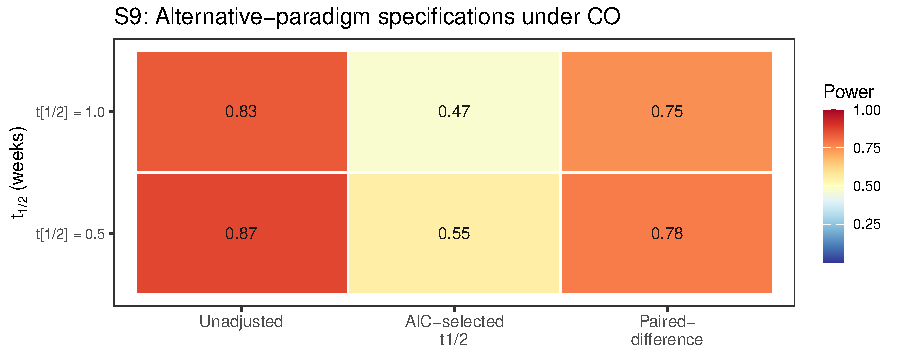
\includegraphics[width=0.75\linewidth]{../../figures/02xs-heatmap-sens-S9} \caption{Block S9: power under the CO design at two true half-lives, same four specifications as block S7.}\label{fig:fig-heatmap-sens-s9}
\end{figure}

It does not, and the result refines rather than overturns Section
4.5's explanation. At \(t_{1/2} = 1.0\) under CO, \texttt{E1} and \texttt{E4} reach
\(0.834\) and \(0.858\); \texttt{E5} and \texttt{E6} reach only \(0.740\) and \(0.770\) on
the joint test, gaps of \(-0.094\) and \(-0.064\) against \texttt{E1}, both
slightly \emph{larger} than the corresponding Hybrid gaps of \(-0.058\) and
\(-0.044\) from block S7. At \(t_{1/2} = 0.5\) the pattern repeats
(\(0.866\)/\(0.880\) for \texttt{E1}/\texttt{E4} against \(0.780\)/\(0.810\) for
\texttt{E5}/\texttt{E6}). The design-driven collinearity mechanism is nonetheless
confirmed directly: \texttt{E6}'s \(\text{bm:}D_{it}\) coefficient, evaluated
alone and ignoring \(\text{bm:}t_{sd}\), is rejected in only \(19.8\%\)
of replicates at the Hybrid reference cell (Table
\ref{tab:tab-s7}) but in \(73.0\%\) under CO at \(t_{1/2} = 1.0\),
nearly matching \texttt{E1}'s own \(83.4\%\). The individual coefficient
becomes far more estimable once \(t_{sd}\) has room to vary. What does
not follow is a joint-test power gain, because the joint test still
spends a second degree of freedom on a term with no counterpart in
the data-generating process: under both architectures examined here,
a single decay parameter governs the entire carryover mechanism, so
\texttt{E5}/\texttt{E6} are structurally over-parameterized relative to the truth
being estimated regardless of how well the design identifies the
extra coefficient. Relieving the collinearity changes \emph{which}
coefficient absorbs the estimation difficulty, not whether the extra
parameter is worth its degree of freedom. A design or DGP in which
the biomarker-treatment interaction's carryover decay genuinely
differs from the main effect's, so that \texttt{bm:L}/\texttt{bm:tsd} corresponds
to a real second parameter rather than a redundant one, remains
untested and is the more fundamental condition under which these
specifications would be expected to win (Section 4.5).

\subsection{A higher-precision check}\label{a-higher-precision-check}

Because a number of the Tier 1 gaps are small, we reran a focused
24-cell grid (OL+BDC design, \(N \in \{35, 70\}\), true half-life
\(\in \{0.5, 1.0\}\)) at 600 trials per cell, all converging, and
compared specifications with a paired McNemar test, considerably
more sensitive than an independent-groups comparison since all three
are fit to the same trials. Type I error across the twelve null
cells fell in \([0.003, 0.053]\), so nominal alpha holds. Paired
McNemar tests place Exposure-weighted ahead of the unadjusted
benchmark at all four alternative cells, by \(+2.3\) to \(+13.7\)
percentage points, with the largest gap at the highest-leverage cell
(\(N = 70\), true \(t_{1/2} = 1.0\) weeks, \(p = 6.6 \times 10^{-17}\))
and \(p \leq 0.015\) at the remaining three, a sharper confirmation
than the Tier 1 grid alone provides.

One scope caveat governs the rerun's third arm. It was produced by
the package's \texttt{lme\_analysis()} routine, whose carryover option
appends time since discontinuation as a linear main effect rather
than the lagged indicator \(L_{it}\) used in the Tier 1 grid. It is
therefore not the Lag-adjusted specification of Section 2.4 and is
not reported as such here. That alternative remains a reasonable
specification we have not evaluated (Section 4.6).

\section{Discussion}\label{discussion}

\subsection{The lagged-treatment term does no work}\label{the-lagged-treatment-term-does-no-work}

The clearest result of this study is a negative one. Adding the
classical lagged-treatment indicator to the analysis model changed
nothing measurable, anywhere in the grid. Across all 216 cells the
mean power difference against the unadjusted benchmark was 0.003
against an MCSE of 0.018, bias, MSE, and coverage agreed to three
decimal places, and the equality held in every sensitivity block and
all five cluster-robust stress cells under both inference
procedures. The strength of this conclusion rests on the design
rather than the grid size. The two specifications estimate the same
coefficient, were fitted to the same simulated datasets under common
random numbers, and differ by exactly one term, so there is no
confounding from a change of estimand, Monte Carlo variation between
arms, or differential test size (both are conservative to the same
degree, Section 3.5). What is left is the term itself, and it
contributed nothing.

The mechanism follows from where the term sits. Carryover damages
the interaction test on two fronts (Section 1). It attenuates the
coefficient, because contaminated occasions are coded as drug-free,
and it inflates the residual variance, because those occasions are
heterogeneous in a way the model does not represent. The lagged
indicator enters only as a nuisance main effect, with no
\(\text{bm:}L_{it}\) product term, so the tested interaction remains
\(\text{bm:}D_{it}\) and the attenuation is untouched. It can in
principle absorb some of the second effect, but evidently absorbs
too little to matter, since it marks a single occasion per
randomization path and is constant thereafter, unable to describe a
graded decline across a two- to four-occasion washout.

A more capable, elapsed-time-indexed nuisance term might succeed
where the crude lagged indicator fails, so we ran a targeted check
on the alternative the reference implementation provides,
\texttt{Sx\ \textasciitilde{}\ bm\ +\ t\ +\ Db\ +\ bm:Db\ +\ tsd}, called the washout-adjusted
specification (\texttt{E4}), across the three designs at true half-lives of
0.5 and 1.0 weeks (\(N = 70\), \(c_{bm} = 0.45\), exponential DGP, 500
replicates). It does slightly better, and the improvement is
instructive rather than material. Type I error is at nominal for
both (mean 0.050 versus 0.045), and power exceeds the benchmark in
all six cells by a mean of 1.3 points (sign test \(p = 0.031\)),
reaching significance under crossover at both half-lives (\(+1.8\),
\(p=0.008\); \(+2.2\), \(p=0.003\)) and OL+BDC at the longer one (\(+2.2\),
\(p=0.015\)), but not Hybrid (\(+1.0\), \(p=0.27\)). The mechanism is
exactly the one Section 2.4 predicts. Point estimates are unchanged,
so nothing about the attenuation is repaired, and the entire effect
runs through the standard error, which only a long enough washout
gives it something to describe. The crossover schedule places
off-drug occasions 2.5 to 10 weeks after discontinuation, against
one to two weeks for Hybrid, so the practical ceiling on what any
carryover nuisance term can deliver is about two percentage points,
and only in long-washout designs, against the nine to eleven points
exposure weighting delivers where it works. This check covers only
the exponential DGP at a single \(N\) and effect size, so it is a
probe rather than a fourth arm, and shares every specification's
structural limitation of entering carryover as a main effect only
(Section 4.5). For practitioners the implication is direct. A
carryover nuisance term of either form should not be expected to
recover meaningful power lost to carryover, and reporting one does
not constitute an effective adjustment for it.

\subsection{The exposure-weighted advantage, and where it fails}\label{the-exposure-weighted-advantage-and-where-it-fails}

The exposure-weighted predictor does help, but conditionally. At
its best cell (Hybrid, \(N = 70\), \(c_{bm} = 0.45\), \(t_{1/2} = 1.0\))
it exceeds the unadjusted benchmark by about 10 points of power
(0.860 versus 0.766, roughly five MCSEs and so not attributable to
chance), confirmed at all four cells of the Section 3.7
high-precision rerun. Under the crossover design it performs
considerably worse (0.488 versus 0.830), apparently because the
within-subject correlation there already carries most of the signal
the decaying predictor was designed to recover, so it gains little
while its down-weighting of off-drug observations works against it.
The recommendation therefore holds only in the two non-crossover
designs, and should not be extended to a crossover trial, where the
unadjusted binary indicator is materially better. That the one
specification addressing attenuation is also the only one to gain
power, while the one addressing only residual variance gains
nothing, suggests attenuation is the mechanism that matters here,
an interpretation consistent with the results rather than a finding
the design isolates directly.

\subsection{What the robustness checks add}\label{what-the-robustness-checks-add}

The Section 3.6 sensitivity blocks show the exposure-weighted
advantage, where it exists, is not fragile. It survives incorrect
decay-shape assumptions (Figure \ref{fig:fig-heatmap-mismatch}),
an incorrectly assumed half-life short of a large over-assumption at
a short true half-life (Figure \ref{fig:fig-sens-s2}), and holds
its five- to eight-point lead across the autocorrelation range
examined (Figure \ref{fig:fig-sens-s1}). One caveat qualifies the
Tier 1 figures throughout. Outside block S2 the analysis-side
half-life is set equal to the data-generating one, granting
Exposure-weighted an oracle no real analyst possesses, so its Tier 1
margins are upper bounds and block S2 gives the more realistic
figure.

\subsection{Dropout matters more than the method}\label{dropout-matters-more-than-the-method}

The finding with the largest practical consequence concerns missing
data, not carryover. When patients drop out (Figure
\ref{fig:fig-sens-s3}), power collapses for all three
specifications together, to between 0.12 and 0.25 at 30\% dropout,
essentially indistinguishable. No specification offers protection,
since each can only organize whatever data remain. MAR dropout is
somewhat worse than MCAR, because the sickest patients, who carry
the most signal, tend to leave first. Retaining patients in the
trial yields considerably more power than any choice among these
three specifications ever could.

\subsection{What analysis is best in which situations, in practice}\label{what-analysis-is-best-in-which-situations-in-practice}

Collecting the findings above into a decision rule rather than a set
of pairwise comparisons:

\begin{itemize}
\tightlist
\item
  \textbf{Covariance moderation (Architecture B), Hybrid or OL+BDC
  design.} Use Exposure-weighted with a CR2 cluster-robust standard
  error. The advantage holds under decay-shape mis-specification
  (Section 3.5), under half-life mis-specification short of a large
  over-assumption (Section 3.6, Block S2), and across the
  autocorrelation range examined (Block S1), and CR2 restores nominal
  Type I error without disturbing the ranking (Block S6, validated at
  \(N \in \{35, 70\}\) in the Hybrid design specifically; OL+BDC was not
  itself stress-tested under CR2). This is the one specification
  recommendation the grid supports without qualification, and it is
  also the only cell type in which Exposure-weighted should be used
  at all.
\item
  \textbf{Crossover (CO) design, any architecture.} Use Unadjusted.
  Exposure-weighted is markedly worse under CO (Section 3.4), and
  Block S9 (below) shows that adding a biomarker-interacted carryover
  term does not rescue it. The classical lagged-treatment remedy adds
  nothing here either (next point), including in the one design where
  its washout is long enough to give it a chance (Section 4.1).
\item
  \textbf{Architecture uncertain, or known to be mean moderation
  (Architecture A).} Use Unadjusted or Lag-adjusted, not
  Exposure-weighted. Its advantage under covariance moderation
  reverses, marginally, under mean moderation (Block S8), so it is
  not a safe default when the biomarker's mechanism of action is not
  established.
\item
  \textbf{Never rely on Lag-adjusted as a carryover remedy.} It is
  statistically indistinguishable from Unadjusted everywhere tested
  in this manuscript, Tier 1 and every Tier 2 block alike (Section
  4.1). If a reviewer or protocol expects some carryover term to be
  present, including it costs nothing measurable, but it should not
  be reported as having adjusted for carryover.
\item
  \textbf{Do not use the biomarker-interacted carryover terms \texttt{E5}/\texttt{E6}}
  under any condition examined (Blocks S7-S9); see below for what
  would need to be true for them to help.
\item
  \textbf{Minimize dropout before optimizing specification choice.} It is
  the single largest lever in the entire grid (Section 4.4), and no
  specification offers any protection against it.
\end{itemize}

\subsubsection{When would a biomarker-interacted carryover term help?}\label{when-would-a-biomarker-interacted-carryover-term-help}

Blocks S7-S9 establish that crossing a carryover term with the
biomarker, \texttt{E5} (\(\text{bm:}L_{it}\)) or \texttt{E6} (\(\text{bm:}t_{sd}\)), does
not recover power at any cell examined. Four conditions would need to
hold simultaneously for that to change; only one has been tested
directly.

\begin{enumerate}
\def\labelenumi{\arabic{enumi}.}
\tightlist
\item
  \textbf{A true DGP where the biomarker-carryover interaction has its own
  decay parameter, separate from the main effect's.} This is the
  structural issue underlying the other three. Under Architecture B,
  \(\text{Cor}(B_i, BR_{it}) = c_{bm} \cdot \phi(t_{sd})\): a single
  decay function governs the entire carryover mechanism.
  \texttt{E5}/\texttt{E6} add a second free parameter that has no counterpart in
  that mechanism, so they are over-parameterized relative to the
  truth being estimated, and two regressors chasing one true degree
  of freedom will generally lose power to a correctly-specified
  single-parameter model. These specifications would be expected to
  help only under a DGP where the interaction's carryover decays at
  a genuinely different rate than the main treatment effect's, for
  instance a biomarker whose predictive value fades slower or faster
  post-discontinuation than the drug's raw pharmacological effect.
  Nothing in this manuscript's DGP does that, in either architecture
  examined, and this condition remains untested; it would require
  modifying the data-generating mechanism itself, not just the
  design or grid.
\item
  \textbf{A design with off-drug occasions spread over a wide, graded
  range of \(t_{sd}\), not the one- to two-week compressed washout
  Hybrid and OL+BDC give.} This is the one condition testable
  without touching the DGP, and Block S9 tests it directly by
  refitting \texttt{E1}, \texttt{E4}, \texttt{E5}, and \texttt{E6} under the CO design (off-drug
  arm spanning 2.5 to 20 weeks) at two true half-lives. The
  mechanism is partially confirmed and partially not. \texttt{E6}'s
  collinearity between \(\text{bm:}D_{it}\) and \(\text{bm:}t_{sd}\),
  severe at the Hybrid reference cell (the \(\text{bm:}D_{it}\)
  coefficient alone rejects in only \(19.8\%\) of replicates there,
  Table \ref{tab:tab-s7}), is substantially relieved under CO
  (\(73.0\%\), close to \texttt{E1}'s own \(83.4\%\) at the same cell): the
  individual coefficient is far more estimable once \(t_{sd}\) has
  room to vary. But the joint-test power gap against \texttt{E1} does not
  close, and is if anything slightly wider under CO than under
  Hybrid (\(-0.094\) versus \(-0.058\) for \texttt{E5}; \(-0.064\) versus
  \(-0.044\) for \texttt{E6}, at \(t_{1/2} = 1.0\); the pattern repeats at
  \(t_{1/2} = 0.5\)). Relieving the collinearity changes which
  coefficient absorbs the estimation difficulty, not whether the
  extra parameter is worth its degree of freedom, which is
  condition 1's point restated with data behind it.
\item
  \textbf{Larger \(N\).} The joint test's power cost is partly a
  finite-sample penalty for the extra estimated parameter, which
  should shrink, though not vanish, as \(N\) grows past the 70 used
  throughout this grid. Untested here.
\item
  \textbf{A short true half-life relative to the available washout
  length}, so there is an actual steep decay for the second term to
  trace rather than one that is already nearly complete or nearly
  flat by the time off-drug data are observed. Block S9's two
  half-lives (\(t_{1/2} \in \{0.5, 1.0\}\) weeks against CO's 2.5- to
  20-week washout) bear on this only weakly, since both are short
  relative to CO's washout length and neither reverses the negative
  result; a true half-life closer to or exceeding the washout length
  itself was not tested.
\end{enumerate}

Taken together, the one lever tested (condition 2) confirms the
mechanism behind \texttt{E6}'s specific failure mode without changing the
practical conclusion: a longer, more graded washout makes the
individual coefficients more estimable but does not overcome the
structural cost of an extra, DGP-unmotivated parameter. Condition 1
is the more fundamental requirement, and it is a statement about the
data-generating process rather than the design or grid, so it is not
addressable within this manuscript's simulation framework without
building a new DGP.

\subsection{Scope, related work, and limits}\label{scope-related-work-and-limits}

This manuscript deliberately narrows the full-scope grid to the
covariance-moderation architecture and to the non-linear decay
forms, in the interest of a self-contained evaluation of manageable
length. The archived full-scope drafts (\texttt{archive/report.Rmd} and
\texttt{archive/report-slim.Rmd}) show that the exposure-weighted advantage
documented here does not carry over to mean moderation, where the
biomarker moderates the mean response directly and Exposure-weighted
is marginally dominated in every design examined. Readers who need
that cross-architecture comparison should consult those drafts
rather than extrapolate from this one. Establishing what the
originally published power values (Section 3.2) were computed under
remains outstanding work.

The crossover tradition surveyed by Jones and Kenward\textsuperscript{\citeproc{ref-jones2014crossover}{4}} would lead one to expect a shape-free lagged
term to outperform a parametric predictor once the decay shape is
mis-specified. Our results do not support that expectation over the
range examined, for two reasons. The exposure-weighted penalty for
an incorrect half-life is too small to be overtaken (Section 3.6),
and more fundamentally the lagged term does not improve on ignoring
carryover at all (Section 4.1), leaving no advantage for
decay-shape mis-specification to erode.

One adjacent specification bounds the negative result of Section
4.1. Every carryover term considered there, lagged and
washout-adjusted alike, enters as a nuisance main effect with no
product against the biomarker, so that finding is that a carryover
\emph{main effect} does not recover the attenuated signal, not that no
shape-free specification can. The natural candidate is a carryover
term interacted with the biomarker, either \texttt{Sx\ \textasciitilde{}\ bm\ +\ t\ +\ Db\ +\ bm:Db\ +\ L\ +\ bm:L} or its washout-adjusted counterpart with \texttt{bm:tsd},
letting the biomarker effect decline across the washout without
committing to a rate. Blocks S7-S9 (Section 3.6) test exactly these
two specifications, under both trial designs and architectures
examined in this manuscript, and find the same negative result
extends to them throughout; Section 4.5 discusses the mechanism and
what conditions would need to hold for that to change. Block S8
further shows the Lag-adjusted null of Section 3.3 replicates under
Architecture A, so it is not an artifact specific to covariance
moderation. Only the Exposure-weighted advantage is
architecture-sensitive, reversing in direction, though not
significantly, under Architecture A (Section 3.6, Block S8).

Two further limitations bound what we can conclude. The numbers
presented here come from a single parameter set calibrated to a
prazosin and PTSD trajectory, so absolute power values should be
read as illustrative and the ranking, itself conditional on trial
design, as the more portable result. And the sensitivity checks vary
one factor at a time and can therefore miss genuine interactions
between factors, for instance between high autocorrelation and heavy
dropout. The one joint check available to us, block S5 in the
full-scope manuscript, revealed no such interaction.

\section{Conclusions}\label{conclusions}

\begin{enumerate}
\def\labelenumi{\arabic{enumi}.}
\item
  \textbf{The lagged-treatment term does nothing.} It never improved on
  ignoring carryover altogether, on any measure, in any design, at
  any half-life, and in every sensitivity block, a clean null given
  the two specifications share an estimand and differ by a single
  term. The term enters as a nuisance main effect only, leaving the
  attenuation of the interaction untouched, and should not be
  reported as an adjustment for carryover.
\item
  \textbf{Exposure weighting helps, but conditionally.} It achieves the
  highest power, about 10 points over the unadjusted benchmark, only
  in the Hybrid and OL+BDC designs, and its lead survives
  mis-specified decay shape and half-life there. Under crossover it
  is markedly worse than the binary indicator (0.488 against 0.830)
  and should not be used. Where used, we recommend a CR2
  cluster-robust standard error (Block S6).
\item
  \textbf{An approximate half-life is adequate, but err short.} A
  fourfold error at a true half-life of one week costs 6.6 points of
  power, so a rough pharmacokinetic estimate suffices in practice.
  The error is asymmetric. Under-assuming drives the predictor
  toward the still-serviceable binary indicator, while over-assuming
  erodes the advantage to a tie. Outside block S2 the analyst is
  granted the true half-life, so the Tier 1 margins are upper
  bounds.
\item
  \textbf{Dropout matters more than the choice of method.} Power falls
  sharply as dropout increases, roughly halving at 20\%, equally
  across all three specifications. Preventing dropout is a more
  effective use of design effort than any choice among them.
\item
  \textbf{The interaction test is somewhat conservative, and correctably
  so.} All three specifications reject slightly less often than
  nominal under the null. A CR2 cluster-robust standard error
  restores the correct rate while recovering modest power, and the
  exposure-weighted advantage is held or widened under CR2 at four
  of five S6 stress cells (Block S6).
\item
  \textbf{This is a narrowed slice of a larger study.} Mean moderation
  and linear decay fall outside this manuscript's scope. The
  archived drafts \texttt{archive/report.Rmd} and \texttt{archive/report-slim.Rmd}
  are the authority on those comparisons and should be consulted
  before generalizing beyond covariance moderation. We also make no
  claim of numerical agreement with the originally published power
  values (Section 3.2).
\item
  \textbf{Biomarker-interacted carryover terms do not help either, and
  the finding is not architecture- or design-specific.} Crossing a
  lagged or washout carryover term with the biomarker, the natural
  elaboration of the negative result in item 1, gives lower power
  than the unadjusted benchmark once evaluated by the joint test
  its extra coefficient requires (Block S7), and the washout form
  additionally destabilizes the interaction coefficient it was
  meant to unbias. Block S8 confirms this negative result, and the
  Lag-adjusted null of item 1, hold under Architecture A as well as
  B, across the full carryover-severity range tested
  (\(t_{1/2} \in \{0, 0.5, 1.0\}\)). Block S9 confirms it does not
  depend on Hybrid's compressed washout either: switching to the
  crossover design, whose off-drug arm gives the interacted terms'
  extra coefficient far more identifying information, relieves the
  specific collinearity that destabilizes the washout form but does
  not close the joint-test power gap, which if anything widens
  slightly. Section 4.5 discusses why: both architectures examined
  here generate carryover from a single decay parameter, so the
  interacted specifications are structurally over-parameterized
  relative to the truth being estimated regardless of how well any
  given design identifies the extra coefficient. Only the
  Exposure-weighted advantage is architecture-sensitive: it reverses
  in direction under Architecture A, a small but real effect at
  \(t_{1/2} = 1.0\) (about 1.5 MCSE), confirming that item 2's
  recommendation is conditional on Architecture B and should not be
  extrapolated to Architecture A.
\end{enumerate}

\section{Conflict of interest}\label{conflict-of-interest}

The authors declare no conflicts of interest.

\section{Funding}\label{funding}

This work received no specific funding.

\section{Data availability statement}\label{data-availability-statement}

The data and code supporting the findings of this study are
available in the pmsimstats-ng project repository. Per-replicate
Monte Carlo outputs and ADEMP-compliant cell-level summaries are
versioned under \texttt{analysis/data/}. Simulation drivers are at
\texttt{analysis/scripts/carryover-sensitivity/}. Exact paths for this
manuscript are listed in the Reproducibility section below.

\section{Reproducibility}\label{reproducibility}

This manuscript was rendered with R 4.6.0 inside the project's
zzcollab Docker container. The production simulation ran under R
4.5.3 (§3.6), with the image hash in \texttt{Dockerfile} and the package
set in \texttt{renv.lock}. The simulation study uses \texttt{nlme} for the continuous-time
linear-mixed analysis, \texttt{parallel} for the 8-core parameter-grid
sweep, and \texttt{data.table} or \texttt{furrr}/\texttt{purrr} in the two simulation
collections. No simulation code runs during knitting, which loads
pre-computed checkpoints only. Each driver sets a master seed
(20260507) and derives per-replicate seeds from it via
\texttt{parallel::mc.set.seed}.

\textbf{Data and code availability.} All simulation outputs, cell-level
summaries, and driver scripts are versioned under
\texttt{analysis/scripts/carryover-sensitivity/} and \texttt{analysis/data/} in
the pmsimstats-ng repository, including the principal factorial, the
S1 to S5 sensitivity blocks, the S6 cluster-robust recalibration,
the washout-adjusted (E4) check of Section 4.1, the high-precision
prototype rerun of Section 3.7, the S7 biomarker-interacted
carryover terms block
(\texttt{09-run-sensitivity-s7.R}, \texttt{output/09-sensitivity-s7.rds}), and the
S8 architecture-sensitivity block, now crossed with half-life
(\texttt{10-run-sensitivity-s8.R}, \texttt{output/10-sensitivity-s8.rds}), and the
S9 CO-design block
(\texttt{14-run-sensitivity-s9.R}, \texttt{output/14-sensitivity-s9.rds}), all
added 2026-08-18 (master seed 20260415, 500 replicates per cell,
Hybrid reference cell except S9, which uses CO). The
five- and six-specification fitters for S7-S9
(\texttt{fit\_spec\_s7}, \texttt{simulate\_cell\_s7}) are appended to
\texttt{simulation-core.R} alongside the Tier 1 \texttt{fit\_spec}/\texttt{fit\_all\_specs}
pair, which they do not modify. Figures
\ref{fig:fig-hendrickson-a} through \ref{fig:fig-hendrickson-c} are
produced from the same \texttt{02-grid-summary.rds} Tier 1 summary as the
headline table, by \texttt{12-hendrickson-heatmap.R}. The corresponding
Tier 2 heatmaps (S1-S4, S7, S8, S9) are produced by
\texttt{13-hendrickson-heatmap-tier2.R} from \texttt{02-sensitivity-summary.rds}
and the S7/S8/S9 output \texttt{.rds} files, and are additional to, not
replacements for, the existing S1-S4 line plots and S7/S8 kable
tables. The grid design and
Morris ADEMP pre-registration are in
\texttt{simulation-grid-plan.md} in the same directory. Superseded
wider-scope drafts are retained under \texttt{archive/}, documented in its
\texttt{README.md}.

\textbf{Specification labels.} The three specifications are stored as
\texttt{E1}, \texttt{E2}, \texttt{E3} and displayed here as Unadjusted, Lag-adjusted, and
Exposure-weighted. The mapping is applied only at display time, by
\texttt{spec-labels.R}, so the stored values and archived outputs are
unaffected. Output archived before 2026-07-31 stores the
specifications as \texttt{A1}, \texttt{A2}, \texttt{A3}. The migration is documented in
\texttt{analysis/report/NOTATION.md}.

\section{References}\label{references}

\protect\phantomsection\label{refs}
\begin{CSLReferences}{0}{1}
\bibitem[\citeproctext]{ref-morris2019simulation}
\CSLLeftMargin{1. }%
\CSLRightInline{Morris TP, White IR, Crowther MJ. Using simulation studies to evaluate statistical methods. \emph{Statistics in Medicine}. 2019;38(11):2074-2102. doi:\href{https://doi.org/10.1002/sim.8086}{10.1002/sim.8086}}

\bibitem[\citeproctext]{ref-hendrickson2020}
\CSLLeftMargin{2. }%
\CSLRightInline{Hendrickson RC, Thomas RG, Schork NJ, Raskind MA. Optimizing aggregated {N}-of-1 trial designs for predictive biomarker validation: Statistical methods and practical considerations. \emph{Frontiers in Digital Health}. 2020;2:13. doi:\href{https://doi.org/10.3389/fdgth.2020.00013}{10.3389/fdgth.2020.00013}}

\bibitem[\citeproctext]{ref-pmsimstats_dgp_architectures2026}
\CSLLeftMargin{3. }%
\CSLRightInline{{pmsimstats team}. Two architectures for simulating biomarker-treatment interactions in aggregated {N}-of-1 trials. Published online 2026.}

\bibitem[\citeproctext]{ref-jones2014crossover}
\CSLLeftMargin{4. }%
\CSLRightInline{Jones B, Kenward MG. \emph{Design and Analysis of Cross-over Trials}. 3rd ed. CRC Press; 2014.}

\bibitem[\citeproctext]{ref-pmsimstats_calibration2026}
\CSLLeftMargin{5. }%
\CSLRightInline{{pmsimstats team}. Type-{I} calibration of fixed-effect interaction tests in linear mixed models: A staged diagnosis of working-covariance mis-specification and a cluster-robust remedy. Published online 2026.}

\end{CSLReferences}

\end{document}
